\chapter{Perancangan}
Berdasarkan analisis yang telah dilakukan, terdapat beberapa hal yang perlu dirancang untuk pembangunan perangkat lunak naive bayes berbasis \textit{hadoop mapreduce}. Pada bab ini akan dijelaskan perancangan yang diperlukan untuk membangun perangkat lunak yaitu perancang-
an antarmuka, diagram kelas rinci, serta rincian metode.
			
\section{Perancangan Antarmuka}
\label{sec:Perancangan Antarmuka}

Perangkat lunak \textit{naive bayes classification} memiliki 6 buah tampilan untuk yang tidak berbasis \textit{MapReduce}, yaitu: (1) \textit{Dashboard} (2) \textit{Input Set Manager} (3) \textit{Renew Model Manager} (4) \textit{Testing Manager} (5) \textit{Classification Manager} (6) \textit{Error Rate Dashboard}. Untuk program yang berbasis \textit{MapReduce} tidak akan memiliki antarmuka yang khusus, karena program hanya perlu dijalankan dengan menggunakan CLI (\textit{command line interface}). Berikut adalah penjelasan dan gambar dari tiap antarmuka yang dirancang:

\subsection{\textit{Dashboard}}
\label{subsec:Dashboard}

\begin{figure}[H]
	\centering
	\includegraphics[scale=0.45]{Mockup/mockup_dashboard_0}
	\caption[input-set-gui-1]{Dashboard}
	\label{fig:input-set-gui-1}
\end{figure}
\textit{Dashboard} dibuat untuk memudahkan user dalam memonitor model NBC yang telah dimasukkan ke dalam perangkat lunak yang dibangun. Berikut penjelasan lebih lanjut mengenai tiap komponen pada rancangan \textit{dashboard} yang dibuat:
\begin{enumerate}
	\item Berisi nama - nama atribut kelas dan total frekeunsi kemunculannya tiap nilai.
	\item Berisi nama - nama atribut prediktor dan frekuensi kemunculannya untuk prediktor bertipe diskrit dan \textit{mean} \verb|&| \textit{sigma} untuk yang bertipe numerik.
	\item \textit{Bayesian model} merupakan model dari NBC yang akan digunakan untuk testing dan klasifikasi. Model ini merupakan model yang langsung di-import dari hasil training di dalam HDFS.
\end{enumerate}

\subsection{\textit{Input Set Manager}}
\label{subsec:Input Set Manager}

\begin{figure}[H]
	\centering
	\includegraphics[scale=0.4]{Mockup/input-set-gui-1}
	\caption[\textit{Input Set Manager}]{\textit{Input Set Manager}}
	\label{fig:Input Set Manager}
\end{figure}
\textit{Input Set Manager} dibuat untuk memudahkan user melakukan input data ke dalam HDFS menggunakan perangkat lunak yang dibuat. Berikut penjelasan lebih lanjut mengenai tiap komponen pada rancangan \textit{Input Set Manager} yang dibuat:
\begin{enumerate}
	\item User dapat memilih tipe model input yang sudah ada dalam HDFS.
	\item Jika ingin membuat tipe model input baru pada HDFS, maka user perlu mengisi kolom ini dan mengisi nama model yang diinginkan.
	\item User dapat memilih file input yang akan dikirimkan ke dalam HDFS. User dapat memilih > 1 file sekaligus.
	\item User dapat memilih file info mengenai file input, yang dikirimkan ke dalam HDFS.
	\item User dapat memilih presentase pembagian data antara data \textit{training} dan data \textit{testing} dari keseluruhan data input yang akan dimasukkan ke dalam HDFS.
	\item Setelah memillih file info, user dapat memilih atribut mana saja yang akan digunakan untuk training. User juga dapat memilih tipe(diskrit/numerik) dari atribut tersebut beserta jenisnya (kelas/prediktor).
\end{enumerate}

\subsection{\textit{Renew Model Manager}}
\label{subsec:Renew Model Manager}

\begin{figure}[H]
	\centering
	\includegraphics[scale=0.45]{Mockup/mockup_renewmodel_manager}
	\caption[\textit{Renew Model Manager}]{\textit{Renew Model Manager}}
	\label{fig:Renew Model Manager}
\end{figure}
\textit{Renew Model Manager} dibuat agar user selalu bisa memperbaharui model NBC pada perangkat lunak yang dibikin.
\begin{enumerate}
	\item User dapat memilih file model NBC hasil dari training dari sistem penyimpanan \textit{local}.
	\item User dapat memilih file model NBC hasil dari training langsung dari HDFS.
\end{enumerate}

\subsection{\textit{Testing Manager}}
\label{subsec:Testing Manager}

\begin{figure}[H]
	\centering
	\includegraphics[scale=0.45]{Mockup/mockup_testing_manager}
	\caption[\textit{Testing Manager}]{\textit{Testing Manager}}
	\label{fig:Testing Manager}
\textit{Testing Manager} dibuat untuk melakukan testing pada model NBC yang sudah di-import ke dalam program sebelumnya.
\end{figure}
\begin{enumerate}
	\item User dapat memilih file input dan file info dari penyimpanan \textit{local} milik user.
	\item User dapat memilih file testing yang sudah ada di dalam HDFS dengan memilih model input direktori pada HDFS.
\end{enumerate}

\subsection{\textit{Classification Manager}}
\label{subsec:Classification Manager}

\begin{figure}[H]
	\centering
	\includegraphics[scale=0.45]{Mockup/mockup_classification_manager}
	\caption[\textit{Classification Manager}]{\textit{Classification Manager}}
	\label{fig:Classification Manager}
\end{figure}
\textit{Classification Manager} dapat digunakan untuk mengklasifikasi satu record input/kasus yang secara langsung diisi sendiri oleh user yang menggunakannya terhadap model NBC yang sudah ada pada perangkat lunak sebelumnya.
\begin{enumerate}
	\item User memilih nilai prediktor untuk kasus baru (prediktor dapat berupa dropdown untuk yang bertipe diskrit dan \textit{number} untuk yang bertipe numerik)
	\item User dapat memilih kelas yang menjadi prediksi sebelumnya dari user untuk diperiksa kebenarannya jika menggunakan program setelah diklasifikasikan menggunakan model NBC yang sudah ada.
	\item Hasil dari klasifikasi yang telah dijalankan.
\end{enumerate}

\subsection{\textit{Error Rate Dashboard}}
\label{subsec:Error Rate Dashboard}

\begin{figure}[H]
	\centering
	\includegraphics[scale=0.45]{Mockup/mockup_errorrate}
	\caption[\textit{Error Rate Dashboard}]{\textit{Error Rate Dashboard}}
	\label{fig:Error Rate Dashboard}
\end{figure}
\textit{Error Rate Dashboard} dibuat untuk memonitor hasil \textit{error rate} yang sudah dihitung setelah menjalani proses testing. 
\begin{enumerate}
	\item \textit{Confusion matrix} untuk setiap atribut kelas.
	\item Error rate yang akan dihasilkan setelah melakukan klasifikasi meliputi: (1)$Accuracy$; (2)$Precision$; (3)$Recall$; (4)$F-Measure$.
\end{enumerate}



\section{Diagram Kelas Lengkap dan Design Pattern}
Berikut adalah penjelasan dari kelas - kelas pada keempat modul yang dibuat beserta penjelasan setiap atribut dan operasi yang dimiliki oleh kelas - kelas tersebut.

\subsection{Diagram Kelas Modul \textit{Train Naive Bayes M-R Based}}
Pada diagram kelas ini terdapat terdapat 2 \textit{package} utama yang akan menjadi inti dari modul ini, salah satunya merupakan \textit{package} yang dimiliki oleh \textit{library} dari \textit{hadoop client} untuk dapat menjalankan proses \textit{mapreduce}. Berikut adalah gambar dari \textit{package - package} tersebut:
\begin{figure}[H]
	\centering
	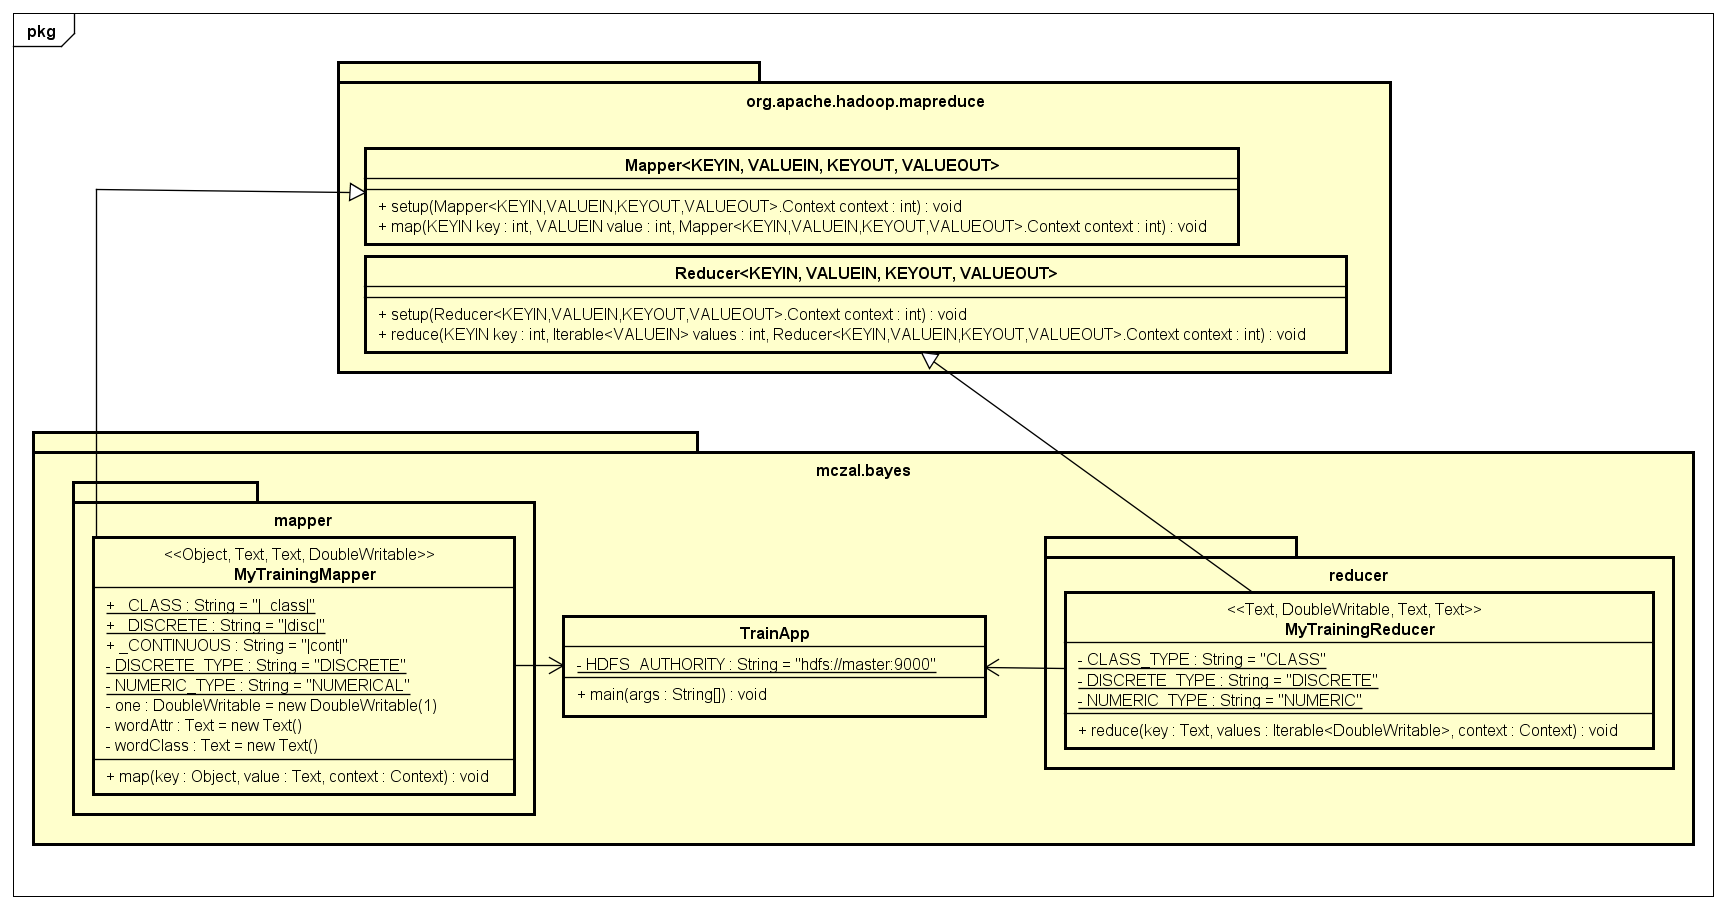
\includegraphics[scale=0.6]{ClassDiagramLengkap/CD_Train_MR}
	\caption[Diagram Kelas \textit{Train Naive Bayes M-R Based}]{\textit{Diagram Kelas Train Naive Bayes M-R Based}}
	\label{fig:Diagram Kelas Modul Kelola Input}
\end{figure}

\paragraph{\textit{Package} $org.apache.hadoop.mapreduce$}
Dalam \textit{package} ini terdapat 2 kelas utama yang akan menjadi kelas \textit{parent} dari kelas \textit{reducer} dan \textit{mapper} yang di-implementasikan.
\begin{enumerate}
	\item{Kelas \textit{Mapper}}\\
	Kelas ini memiliki 4 buah \textit{generic types}\footnote{A generic type is a generic class or interface that is parameterized over types \cite{GenericTypeJavaOracle}} yang perlu di-implementasikan pada kelas yang mengimplementasi method ini. Parameter \textit{generic types} tersebut antara lain adalah:
	\begin{itemize}
		\item{\textit{KEYIN}}\\
		Kelas ini merupakan tipe kelas yang akan menjadi \textit{key} masukan pada proses Map untuk program \textit{Mapreduce} yang dibuat.		
		\item{\textit{VALUEIN}}\\
		Merupakan tipe kelas yang akan menjadi \textit{value} dari masukan pada proses Map untuk program \textit{Mapreduce} yang dibuat.
		\item{\textit{KEYOUT}}\\
		Merupakan tipe kelas yang akan menjadi \textit{key} keluaran pada proses Map untuk program \textit{Mapreduce} yang dibuat.
		\item{\textit{VALUEOUT}}\\
		Merupakan tipe kelas yang akan menjadi \textit{value} keluaran pada proses Map untuk program \textit{Mapreduce} yang dibuat.
	\end{itemize}
	
	\item{Kelas \textit{Reducer}}\\
	Kelas ini memiliki 4 buah \textit{generic types} yang perlu di-implementasikan pada kelas yang mengimplementasi method ini. Parameter \textit{generic types} tersebut antara lain adalah:
	\begin{itemize}
		\item{\textit{KEYIN}}\\
		Kelas ini merupakan tipe kelas yang akan menjadi \textit{key} masukan pada proses \textit{Reduce} untuk program \textit{Mapreduce} yang dibuat.		
		\item{\textit{VALUEIN}}\\
		Merupakan tipe kelas yang akan menjadi \textit{value} dari masukan pada proses \textit{Reduce} untuk program \textit{Mapreduce} yang dibuat.
		\item{\textit{KEYOUT}}\\
		Merupakan tipe kelas yang akan menjadi \textit{key} keluaran pada proses \textit{Reduce} untuk program \textit{Mapreduce} yang dibuat.
		\item{\textit{VALUEOUT}}\\
		Merupakan tipe kelas yang akan menjadi \textit{value} keluaran pada proses \textit{Reduce} untuk program \textit{Mapreduce} yang dibuat.
	\end{itemize}
\end{enumerate}

\paragraph{\textit{Package} $mczal.bayes$}
Dalam \textit{package} ini terdapat beberapa \textit{package} lagi dan kelas - kelas yang akan dijadikan implementasi dari kelas \textit{Mapper} dan \textit{Reducer} pada package \textit{org.apache.hadoop.mapreduce} untuk proses \textit{MapReduce}.
\begin{enumerate}
	\item{Kelas \textit{TrainApp}}\\
	Kelas ini merupakan kelas utama(\textit{main class}) yang akan dijalankan pertama kali program ini dieksekusi. Kelas ini memiliki 1 atribut \textit{static} dan 1 method \textit{main}.
	\begin{enumerate}
		\item Atribut \verb|HDFS_AUTHORITY| \\
		Atribut ini bertipe \textit{String} dan memiliki \textit{modifier} \textit{static} dan \textit{final} agar nilainya tidak dapat diubah - ubah. Inisialisasi pertama dari atribut ini adalah: \verb|"hdfs://master:9000"|. \verb|"hdfs://master:9000"| merupakan url dari node master yang digunakan untuk dapat berkomunikasi dengan node master pada lingkungan \textit{hadoop}. Atribut ini digunakan untuk \textit{request} operasi baca file \textit{meta.info} pada HDFS.
		
		\item Operasi \verb|main|\\
		Operasi ini akan menjadi operasi pertama yang dijalankan ketika melakukan eksekusi program mapreduce pada modul ini. Operasi ini akan men-\textit{set} kelas \textit{mapper} dan kelas \textit{reducer} yang akan digunakan serta variabel - variabel yang perlu dikirimkan kepada tiap node yang dibutuhkan oleh mereka.
	\end{enumerate}

	\item{Kelas \textit{MyTrainingMapper}}\\
	Kelas ini merupakan kelas turunan dari kelas \textit{Mapper} yang ada pada package \verb|org.apache.hadoop.mapreduce|. \textit{Generic type} kelas parent dari kelas ini adalah:
	\begin{enumerate}
		\item{Object} merupakan tipe \textit{key} masukan dari proses \textit{map}.
		\item{Text} merupakan tipe \textit{key} masukan dari proses \textit{map}. Karena, data masukan akan berupa \textit{string}.
		\item{Text} merupakan tipe \textit{key} keluaran dari proses \textit{map}. Karena, \textit{key} pada hasil dari fase \textit{map} akan mengeluarkan data yang bertipe \textit{string}.
		\item{DoubleWritable} merupakan tipe \textit{value} keluaran dari proses \textit{map}. Karena, \textit{value} keluaran pada proses \textit{map} akan berisi jumlah frekuensi atau nilai dari atribut prediktor-numerik yang bertipe numerik.
	\end{enumerate}
	Kelas ini memiliki 8 atribut. Diantaranya adalah:
	\begin{enumerate}
		\item \verb|_CLASS| merupakan atribut bertipe \textit{string} yang memiliki \textit{modifier} \textit{static} dan \textit{final}. Atribut ini memiliki nilai inisialisasi awal = $"|$\verb|_|$class|"$ yang akan digunakan untuk membedakan bahwa data keluaran yang memiliki string berisi $"|$\verb|_|$class|"$ merupakan data keluaran yang akan digunakan untuk menghitung jumlah frekuensi dari kemunculan atribut bertipe kelas.
		\item \verb|_DISCRETE| merupakan atribut bertipe \textit{string} yang memiliki \textit{modifier} \textit{static} dan \textit{final}. Atribut ini memiliki nilai inisialisasi awal = $"|disc|"$ yang akan digunakan untuk membedakan bahwa data keluaran yang memiliki string berisi $"|disc|"$ merupakan data keluaran yang akan digunakan untuk menghitung jumlah frekuensi dari kemunculan atribut prediktor bertipe diskrit berdasarkan atribut kelas tertentu.
		\item \verb|_CONTINUOUS| merupakan atribut bertipe \textit{string} yang memiliki \textit{modifier} \textit{static} dan \textit{final}. Atribut ini memiliki nilai inisialisasi awal = $"|cont|"$ yang akan digunakan untuk membedakan bahwa data keluaran yang memiliki string berisi $"|cont|"$ merupakan data keluaran yang akan digunakan untuk mencatat nilai dari atribut numerik berdasarkan atribut kelas tertentu.
		\item \verb|DISCRETE_TYPE| merupakan atribut bertipe \textit{string} yang memiliki \textit{modifier} \textit{static} dan \textit{final}. Atribut ini memiliki nilai inisialisasi awal = $"DISCRETE"$ yang akan digunakan untuk membedakan bahwa data input setelah displit dengan regex ',' pada indeks tertentu memiliki info bertipe diskrit.
		\item \verb|NUMERIC_TYPE| merupakan atribut bertipe \textit{string} yang memiliki \textit{modifier} \textit{static} dan \textit{final}. Atribut ini memiliki nilai inisialisasi awal = $"NUMERICAL"$ yang akan digunakan untuk membedakan bahwa data input setelah displit dengan regex ',' pada indeks tertentu memiliki info bertipe numerik.
		\item \verb|one| merupakan atribut bertipe \textit{DoubleWritable} yang memiliki \textit{modifier} \textit{static}. Atribut ini memiliki nilai inisialisasi awal = integer bernilai 1 yang akan digunakan untuk mencatat tiap kemunculan atribut prediktor terhadap atribut kelas tertentu yang sedang diperiksa dengan jumlah kemunculan sebanyak 1.
		\item \verb|wordAttr| merupakan atribut bertipe \textit{Text} yang memiliki \textit{modifier} \textit{static}. Atribut ini akan digunakan untuk mencatat tiap atribut prediktor yang akan ditulis menjadi \textit{output key} untuk perhitungan probabilitas posterior dari atribut tertentu pada atribut kelas tertentu.
		\item \verb|wordClass| merupakan atribut bertipe \textit{Text} yang memiliki \textit{modifier} \textit{static}. Atribut ini akan digunakan untuk mencatat tiap kemunculan atribut kelas tertentu dan akan ditulis menjadi \textit{output key} untuk perhitungan frekuensi atribut kelas.
	\end{enumerate}
	Kelas ini memiliki 1 buah operasi. Operasi tersebut adalah operasi \textit{map(key : Object, value : Text, context : Context) : void} yang akan melakukan operasi pada fase map untuk proses training pada modul ini. Seperti yang digambarkan pada DFD sebelumnya, proses ini akan melakukan perhitungan jumlah frekuensi kemunculan tiap atribut. Terkecuali untuk atribut prediktor yang bertipe numerik, operasi ini akan mengeluarkan kembali nilai yang dibaca dari input.
	
\begin{algorithm}[H]
\caption{NBC Model Map Algorithm}\label{alg:NBCGenMap}
\begin{algorithmic}[1]
\Procedure{Map}{$key,value,context$}\Comment{Map function}
\State $ $\verb|_|$CLASS \gets "|$\verb|_|$class|"$
\State $ $\verb|_|$DISCRETE \gets "|disc|"$
\State $ $\verb|_|$CONTINUOUS \gets "|cont|"$
\State $ one \gets 1$
\State $ NUMERIC$\verb|_|$TYPE \gets "NUMERICAL"$
\State $ DISCRETE$\verb|_|$TYPE \gets "DISCRETE"$

\State $ countColumn \gets getInputColumnCount$
\State $ inputSplit[] \gets value.split(',')$
\If{inputSplit.length != countCols}\Comment{Ignoring missing values}
	\State \Return
\EndIf

\State $classConf \gets getClassInfo$\Comment{get class info from meta.info}
\State $classSplitConf[] \gets classConf.split(";")$

\State $attrConf \gets getAttributeInfo$\Comment{get predictor info from meta.info}
\State $attrSplitConf[] \gets attrConf.split(";")$

\State $checkerClassPrior \gets classSplitConf.length$
%\For $i \gets 0$ \To $attrSplitConf.length$ \Do
\For{$i \gets 0$ \textbf{to} $attrSplitConf.length$}	
	\If{$attrSplitConf[i].split(",")[2].equals(DISCRETE_TYPE)$}
		%\For $j \gets 0$ \To $classSplitConf.length$ \Do
		\For{$j \gets 0$ \textbf{to} $classSplitConf.length$}	
			\State $currKey \gets $\verb|_| $DISCRETE + attrSplitConf[i].split(",")[0]
              + "," + inputSplit[Integer.parseInt(attrSplitConf[i]
              .split(",")[1])]
              + "," + classSplitConf[j].split(",")[0]
              + "," + inputSplit[Integer.parseInt(classSplitConf[j]
              .split(",")[1])];$
          	\State $wordAttr.set(currKey);$
          	\State $context.write(wordAttr, one)$
		\EndFor
	\EndIf
\EndFor

\EndProcedure
\end{algorithmic}
\end{algorithm}
	
	\item{Kelas \textit{MyTrainingReducer}}\\
	Kelas ini merupakan kelas turunan dari kelas \textit{Reducer} pada \textit{package org.apache.hadoop.mapreduce}. \textit{Generic type} kelas parent dari kelas ini adalah: 
	\begin{enumerate}
		\item Text merupakan tipe \textit{key} masukan dari proses \textit{reduce} yang dikirim dari proses sebelumnya yaitu proses \textit{map}
		\item DoubleWritable merupakan tipe \textit{value} masukan dari proses \textit{reduce} yang dikriim dari proses sebelumnya yaitu proses \textit{map}.
		\item Text merupakan tipe \textit{key} keluaran dari proses \textit{reduce}. Karena data keluaran berupa model NBC akan memiliki key berisi string.
		\item Text merupakan tipe \textit{value} keluaran dari proses \textit{reduce}. Karena data keluaran berupa model NBC akan memiliki \textit{value} berisi string.
	\end{enumerate}
	Kelas ini memiliki 3 atribut yang memiliki \textit{modifier} \textit{static} dan \textit{final}. Atribut tersebut diantaranya adalah:
	\begin{enumerate}
		\item \verb|CLASS_TYPE| merupakan atribut bertipe string yang memiliki nilai inisialisasi awal = \textit{"CLASS"}. Atribut ini akan digunakan sebagai pembeda pada data keluaran yang merupakan atribut kelas.
				
		\item \verb|DISCRETE_TYPE| merupakan atribut bertipe string yang memiliki nilai inisialisasi awal = \textit{"DISCRETE"}. Atribut ini akan digunakan sebagai pembeda pada data keluaran yang merupakan atribut prediktor bertipe diskrit.

		\item \verb|NUMERIC_TYPE| merupakan atribut bertipe string yang memiliki nilai inisialisasi awal = \textit{"NUMERIC"}. Atribut ini akan digunakan sebagai pembeda pada data keluaran yang merupakan atribut prediktor bertipe numerik.
	\end{enumerate}
	
	Kelas ini memiliki 1 buah operasi. Operasi tersebut adalah operasi \textit{reduce(key : Text, values : Iterable<DoubleWritable>, context : Context) : void} yang akan melakukan operasi pada fase reduce untuk proses training pada modul ini. Seperti yang digambarkan pada DFD sebelumnya, proses ini akan melakukan akumulasi dari tiap perhitungan jumlah frekuensi kemunculan tiap value yang memiliki key yang sama. Terkecuali untuk atribut prediktor yang bertipe numerik, operasi ini akan menghitung nilai rata - rata dari tiap value pada key tersebut dan lalu dilanjutkan menghitung nilai standar deviasi pada probabilitas posterior atribut numerik tersebut.
	
	
\begin{algorithm}[H]
\caption{NBC Model Reduce Algorithm}\label{alg:NBCGenReduce}
\begin{algorithmic}[1]
\Procedure{Reduce}{$key,values[],context$}\Comment{Reduce function}

\State \verb|CLASS_TYPE| $\gets$ \texttt{"CLASS"}
\State \verb|DISCRETE_TYPE| $\gets$ \texttt{"DISCRETE"}
\State \verb|NUMERIC_TYPE| $\gets$ \texttt{"NUMERIC"}

\State \texttt{sum} $\gets 0$
\State \texttt{count} $\gets 0$
\State \texttt{caches} $\gets$ \texttt{List<Double>}

\ForAll{\texttt{value} $\in$ \texttt{values}}
	\State \texttt{caches.add(value)}
	\State \texttt{sum} $+=$ \texttt{value}
	\State \texttt{count}$++$
\EndFor

\If{\texttt{key.type} $\gets$ \texttt{discrete}}

\State \texttt{splitter} $\gets$ \texttt{key.split("|")[2]}
\State \texttt{result} $\gets$ \texttt{splitter + "," + sum + "|" +}\verb|DISCRETE_TYPE|
\State \texttt{write(result,"")}

\ElsIf{\texttt{key.type} $\gets$ \texttt{class}}

\State \texttt{splitter} $\gets$ \texttt{key.split("|")[2]}
\State \texttt{result} $\gets$ \texttt{splitter + "," + sum + "|" +}\verb|CLASS_TYPE|
\State \texttt{write(result,"")}

\ElsIf{\texttt{key.type} $\gets$ \texttt{contiuous}}

\State \texttt{mean} $\gets$ \texttt{sum/count}
\State \texttt{calcTemp} $\gets$ \texttt{0.0}

\ForAll{\texttt{c} $\in$ \texttt{caches}}
	\State \texttt{calcTemp} $+= (c - mean)^2$
\EndFor

\State \texttt{calcTemp} $\gets$ \texttt{calcTemp * (1/count)}
\State \texttt{sigma} $\gets calcTemp^{0.5}$
\State \texttt{result} $\gets$  \texttt{key.split("|")[2]}
\State \texttt{write(result, ";" + mean + "|" + sigma + "|" +)}\verb|NUMERIC_TYPE|

\EndIf

\EndProcedure
\end{algorithmic}
\end{algorithm}
	
\end{enumerate}

\subsection{Diagram Kelas Modul \textit{Testing Naive Bayes M-R Based}}
Pada diagram kelas ini terdapat 1 kelas utama(\textit{main}) yang akan dijalankan pertama kali saat program dieksekusi dan 3 package utama yang merupakan implementasi dari modul \textit{testing naive bayes}. Untuk kelas yang berfungsi sebagai \textit{mapper} dan \textit{reducer} pada modul ini, sama dengan diagram kelas pada modul "\textit{Training Naive Bayes M-R Based}" merupakan kelas implementasi(kelas turunan) dari 2 kelas Mapper dan Reducer milik hadoop pada package \verb|org.apache.hadoop.mapreduce|. Karena bentuk relasi-nya sama persis dengan yang ada pada modul "\textit{Training Naive Bayes M-R Based}", pada modul ini tidak akan digambarkan relasi kelas mapper dan reducer dengan 2 kelas parent milik \textit{library hadoop}.

\subsubsection{Kelas \textit{Main}}
\begin{figure}[H]
	\centering
	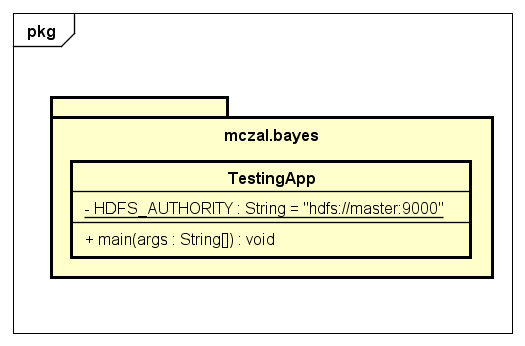
\includegraphics[scale=0.7]{ClassDiagramLengkap/CD_Test_Main}
	\caption[Diagram Kelas Modul \textit{Testing: Main}]{Diagram Kelas Modul \textit{Testing: Main}}
	\label{fig:Diagram Kelas Modul Testing: Main}
\end{figure}
	Kelas \textit{TestingApp} ini merupakan kelas utama(\textit{main class}) yang akan dijalankan pertama kali program \textit{MapReduce} ini dieksekusi. Kelas ini memiliki 1 atribut \textit{static} dan 1 method \textit{main}.
	\begin{enumerate}
		\item Atribut \verb|HDFS_AUTHORITY| \\
		Atribut ini bertipe \textit{String} dan memiliki \textit{modifier} \textit{static} dan \textit{final} agar nilainya tidak dapat diubah - ubah. Inisialisasi pertama dari atribut ini adalah: \verb|"hdfs://master:9000"|. \verb|"hdfs://master:9000"| merupakan url dari node master yang digunakan untuk dapat berkomunikasi dengan node master pada lingkungan \textit{hadoop}. Atribut ini digunakan untuk \textit{request} operasi baca file \textit{meta.info} pada HDFS.
		
		\item Operasi \verb|main|\\
		Operasi ini akan menjadi operasi pertama yang dijalankan ketika melakukan eksekusi program mapreduce pada modul ini. Operasi ini akan men-\textit{set} kelas \textit{mapper} dan kelas \textit{reducer} yang akan digunakan serta variabel - variabel yang perlu dikirimkan kepada tiap node yang dibutuhkan oleh mereka.
	\end{enumerate}


\subsubsection{\textit{Package Base}}
\begin{figure}[H]
	\centering
	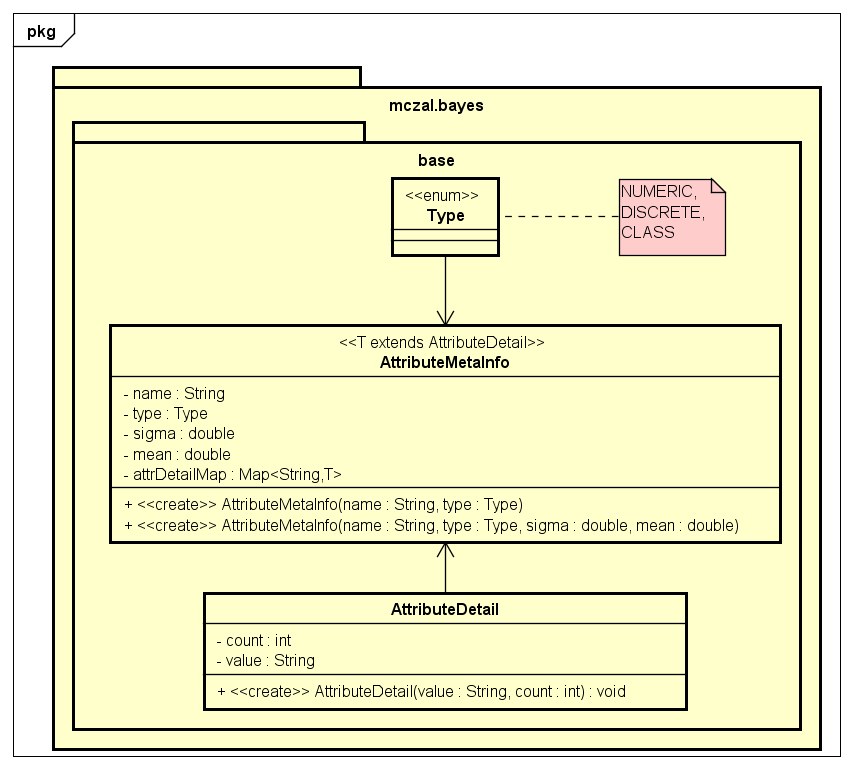
\includegraphics[scale=0.64]{ClassDiagramLengkap/CD_Test_BASE}
	\caption[Diagram Kelas Modul \textit{Testing: Package Base}]{Diagram Kelas Modul \textit{Testing: Package Base}}
	\label{fig:Diagram Kelas Modul Testing: Package Base}
\end{figure}

Pada package ini terdapat 3 kelas utama yang akan menjadi kelas \textit{parent}(\textit{superclass}) dari kelas - kelas yang akan mengimplementasikan-nya. Kelas - kelas parent pada package ini dibuat untuk memenuhi konsep inheritance yang baik dan menghindari terjadinya duplikasi kode pada kelas - kelas terseubt. Kelas - kelas ini juga akan meminimumkan kode yang nantinya dibuat. Berikut adalah penjelasan lebih lanjut mengenai tiap kelas serta atribut dan operasi yang dimilikinya:

\begin{enumerate}
	\item \texttt{Enum}\footnote{Enum adalah sebuah tipe data yang nilainya hanya terbatas dari pilihan nilai-nilai yang telah didefinisikan terlebih dahulu. \textit{Enumeration} di Java baru diperkenalkan pada versi Java 5.} \textit{Type}\\ ini berisi:
	\begin{enumerate}
		\item NUMERIC
		\item DISCRETE
		\item CLASS
	\end{enumerate}
	\textit{Enum} ini akan digunakan sebagai pengenal tipe dari tiap atribut yang ada pada model NBC.
	
	\item{Kelas \texttt{AttributeMetaInfo}}\\
	Kelas ini memiliki 1 buah parameter \textit{generic type} yang perlu diimplementasikan pada kelas yang akan menjadi turunan dari kelas ini. \textit{Generic type} pada kelas ini harus merupakan turunan dari kelas \texttt{AttributeDetail}. Kelas ini akan mencatat seluruh atribut(jenis: prediktor,kelas;tipe: numerik,diskrit) yang ada pada model NBC. Atribut yang akan dimiliki oleh kelas ini merupakan atribut yang merepresentasikan atribut pada model NBC secara umum. Atribut - atribut pada kelas ini adalah:
	\begin{enumerate}
		\item{\texttt{name}}\\ 
		Atribut ini bertipe \texttt{string} yang akan merepresentasikan nama dari atribut pada model NBC.

		\item{\texttt{type}}\\
		Atribut ini bertipe \texttt{Enum Type} yang akan merepresentasikan jenis dari atribut pada model NBC.

		\item{\texttt{sigma}}\\
		Atribut ini bertipe \texttt{double} yang akan merepresentasikan nilai standar deviasi dari keseluruhan data atribut ini pada model NBC jika dan hanya jika tipe dari atribut ini merupakan numerik. Jika tidak, maka nilai atribut ini akan selalu dikosongkan.

		\item{\texttt{mean}}\\
		Atribut ini bertipe \texttt{double} yang akan merepresentasikan nilai rata - rata dari keseluruhan data atribut ini pada model NBC jika dan hanya jika tipe dari atribut ini merupakan numerik. Jika tidak, maka nilai atribut ini akan selalu dikosongkan.

		\item{\texttt{attrDetailMap}}\\
		Atribut ini bertipe \texttt{Map} dengan \texttt{key=string} dan \texttt{value=T(generic type)} yang akan merepresentasikan kumpulan dari semua nilai yang dimiliki oleh atribut ini jika dan hanya jika tipe dari atribut ini merupakan diskrit atau atribut kelas. Jika tidak, maka nilai atribut ini akan selalu dikosongkan.
	\end{enumerate}
	
	Kelas ini menerima 2 buah operasi konstruktor untuk membuat instansiasi dan menginisialisasi nilai - nilai dari atribut di dalamnya. Konstruktor tersebut antara lain adalah:
	\begin{enumerate}
		\item \texttt{AttributeMetaInfo(name : String, type : Type)}\\
		Konstruktor ini digunakan untuk menginisialisasi atribut tanpa mengisi nilai dari atribut \texttt{sigma} dan \texttt{mean}. Konstruktor ini biasa digunakan untuk atribut bertipe \textit{non-numerik}.
		\item \texttt{AttributeMetaInfo(name : String, type : Type, sigma : double, mean : double)}\\
		Konstruktor ini digunakan untuk menginisialisasi atribut dengan mengisi seluruh atribut yang ada, kecuali \texttt{attrDetailMap}. Konstruktor ini biasa digunakan untuk atribut bertipe numerik.
		
	\end{enumerate}
	
	\item{Kelas \texttt{AttributeDetail}}\\
	Kelas ini akan merepresentasikan tiap nilai diskrit dari atribut diskrit/kelas yang ada pada model NBC. Selain mencatat nama dari nilai diskrit atribut diskrit/kelas pada NBC, kelas ini juga akan mencatat jumlah frekuensi dari atribut ini pada model NBC.
	Kelas ini memiliki 2 atribut dan 1 operasi konstruktor, diantaranya adalah:
	\begin{enumerate}
		\item Atribut \texttt{count} bertipe \texttt{integer} yang akan digunakan untuk mencatat jumlah frekuensi dari kemunculan nilai atribut ini.
		\item Atribut \texttt{value} bertipe \texttt{string} yang akan digunakan untuk mencatat nama dari nilai diskrit instansiasi dari kelas ini.
		\item Operasi konstruktor \texttt{AttributeDetail(value : String, count : int): void} akan menginisialisasi nilai awal seluruh atribut yang dimiliki oleh kelas ini pada saat instansiasi objek dari kelas ini.
	\end{enumerate} 
	
\end{enumerate}

\subsubsection{\textit{Package Mapper}}
\begin{figure}[H]
	\centering
	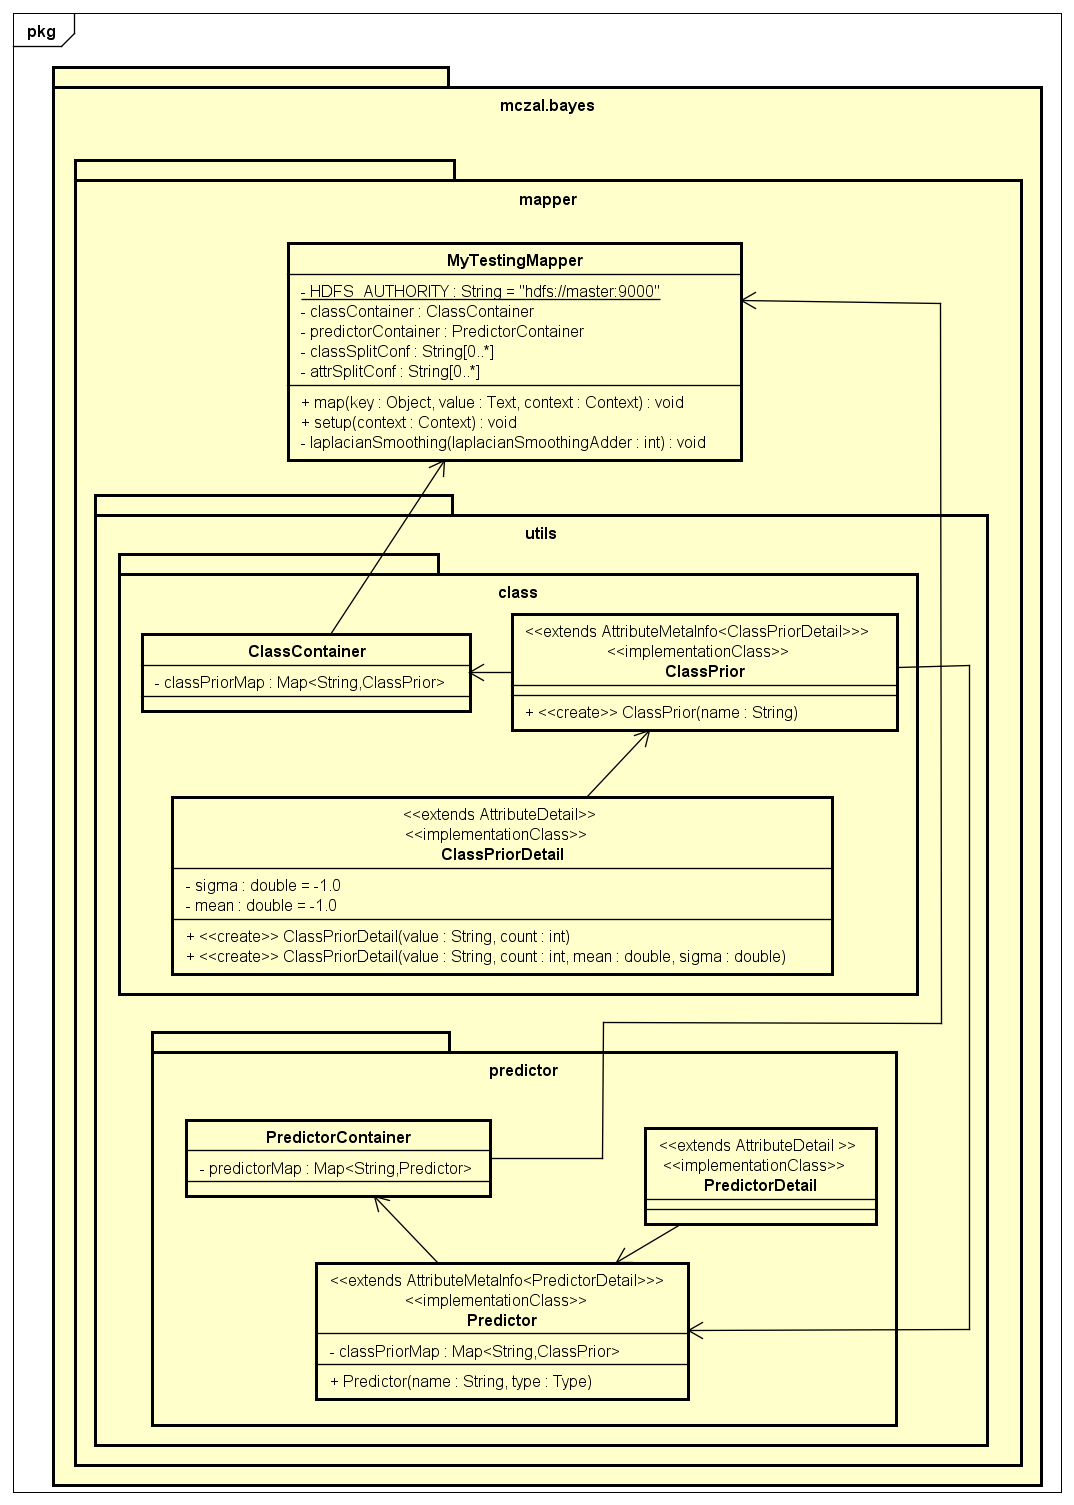
\includegraphics[scale=0.6]{ClassDiagramLengkap/CD_Test_Mapper}
	\caption[Diagram Kelas Modul \textit{Testing: Package Mapper}]{Diagram Kelas Modul \textit{Testing: Package Mapper}}
	\label{fig:Diagram Kelas Modul Testing: Package Mapper}
\end{figure}
Pada package ini terdapat 7 kelas utama yang akan digunakan untuk melakukan proses pada fase \textit{map} pada modul testing. Berikut merupakan penjelasan tiap package dan kelas - kelas yang ada pada \texttt{Package mapper}:
\begin{enumerate}
	\item{Kelas \texttt{MyTestingMapper}}\\
	Kelas ini merupakan kelas utama yang akan dijalankan pada proses map. Kelas ini memiliki 5 atribut dan 3 operasi yang akan digunakan untuk dapat melakukan operasi pada fase map secara keseluruhan. Berikut merupakan penjelasan mengenai atribut dan operasi pada kelas ini:
	\begin{itemize}
		\item{Atribut}
		\begin{enumerate}
			\item{\verb|HDFS_AUTHORITY|}\\
		Atribut ini bertipe \textit{String} dan memiliki \textit{modifier} \textit{static} dan \textit{final} agar nilainya tidak dapat diubah - ubah. Inisialisasi pertama dari atribut ini adalah: \verb|"hdfs://master:9000"|. \verb|"hdfs://master:9000"| merupakan url dari node master yang digunakan untuk dapat berkomunikasi dengan node master pada lingkungan \textit{hadoop}. Atribut ini digunakan untuk \textit{request} operasi baca file \textit{meta.info} dan model NBC pada HDFS.
		
		\item{\texttt{classContainer}}\\
		Atribut ini bertipe \texttt{ClassContainer} yang akan menyimpan seluruh model atribut NBC yang merupakan atribut kelas. 

		\item{\texttt{predictorContainer}}\\
		Atribut ini bertipe \texttt{PredictorContainer} yang akan menyimpan seluruh model atribut NBC yang merupakan atribut prediktor. 

		\item{\texttt{classSplitConf}}\\
		Atribut ini bertipe \texttt{array of string} yang menyimpan seluruh keterangan mengenai field - field yang merupakan atribut bertipe kelas yang digunakan pada model NBC. Keterangan yang disimpan pada atribut ini adalah: (1) nomor indeks; (2) name field; (3) jenis atribut. 

		\item{\texttt{attrSplitConf}}\\
		Atribut ini bertipe \texttt{array of string} yang menyimpan seluruh keterangan mengenai field - field yang merupakan atribut bertipe prediktor yang digunakan pada model NBC. Keterangan yang disimpan pada atribut ini adalah: (1) nomor indeks; (2) name field; (3) jenis atribut.
		
		\end{enumerate}
		
		\item{Operasi}
		\begin{enumerate}
			\item{\texttt{map(}}
			Operasi ini akan melakukan proses pada fase \textit{map} untuk proses testing pada modul ini. Proses yang dilakukan akan meliputi perhitungan nilai probabilitas posterior untuk setiap input pada value. Proses perhitungan tersebut akan dibagi menjadi 2 proses yang terpisah untuk atribut numerik dan diskrit. Setelah diketahui hasilnya, lalu akan disimpan hasil-nya untuk dijadikan keluaran pada operasi ini. Berikut merupakan \texttt{pseudo-code} pada operasi ini:
			\begin{algorithm}[H]
			\caption{NBC Testing algorithm}\label{alg:NBCTestMap}
			\begin{algorithmic}[1]
			\Procedure{Map}{$key,value,context$}\Comment{Map function}
			\State \texttt{input} $\gets$ \texttt{value.toString().trim().split(",")}
			\State \texttt{allResults} $\gets$ \texttt{List<String>}\Comment{\texttt{Format:[CN|CV|Res|Act]}}
			\ForAll{$(classIdx,className) \in classSplitConf$}
				\State $currInClassValue \gets input[classIdx]$
				\State $classPrior \gets classContainer[className]$
				\State $allClassResult \gets ListOfString$\Comment{seluruh hasil dari tiap kelas}
				\ForAll{$(classPriorDetail) \in classPrior$}
					\State $currClassAllPredictorResult \gets 1.0$
					\State $flag \gets 0$
					\State $outer:$
					
					\ForAll{$(attrIdx,attrName,attrType) \in attrSplitConf$}
						\State $currInAttrValue \gets input[attrIdx]$	
						
						\If{$attrType \gets $discrete}
							\State $predictor \gets predictorContainer[attrName]$
							\State $predDetail \gets predictor.getDetail[currInAttrValue]$
							\State $countDividend \gets classPriorDetail.getCount$
							\State $divClassPrior \gets predidctor.getClassPrior[className]$
							\State $divClassPriorDetail \gets divClassPrior.getDetail[classPriorDetail]$
							\State $divisor \gets divClassPriorDetail.getCount$
							\State $currRes \gets (countDividend) / (divisor)$
							\State $currClassAllPredictorResult *= currRes$
						\ElsIf{$attrType \gets $numeric}
							\State $predictor \gets predictorContainer[attrName]$
							\State $mean \gets classPriorDetail.getMean$
							\State $sigma \gets classPriorDetail.getSigma$
							\State $divisor \gets \sqrt{2.0 * \Pi * sigma}$
							\State $powerDividend \gets currInAttrValue - mean)^2 * -1$
							\State $powerDivisor \gets 2.0 * \frac{sigma}{2}$
							\State $resPower \gets powerDividend / powerDivisor$
							\State $currRes \gets (1/divisor) * Math.E^{resPower}$
							\State $currClassAllPredictorResult *= currRes$
						\EndIf
						
						\State $currClassCount \gets classPriorDetail.getCount()$
						\State $allCurrClassCount \gets 0.0$

						\ForAll{$x \in classPrior.getDetail$}
							\State $allCurrClassCount += x.getCount$
						\EndFor
												
						\State $currClassAllPredictorResult *= (currClassCount/allCurrClassCount)$
						\State $allClassResult.add(currClassAllPredictorResult)$
					\EndFor					
					
				\EndFor
				
				\State $maxClass \gets ""$
				\State $checker \gets Double.MIN$\verb|_|$VALUE$
				\State $divisorNorm \gets 0.0$
				
				\ForAll{$result \in allClassResult$}
					\State $divisorNorm += result.currentVal$
					\If{$checker < currentVal$}
						\State $checker = currentVal$
          				\State $maxClass = s$
					\EndIf
				\EndFor
				
				\State $allResults.add(maxClass)$
				
			\EndFor
			
			\ForAll{$result \in allResults$}
				\State $write(result)$
			\EndFor

			\EndProcedure
			\end{algorithmic}
			\end{algorithm}
			
			\item{\texttt{setup(}}
			Operasi ini akan melakukan pembacaan model NBC yang sudah dibuat pada proses sebelumnya pada modul training dalam HDFS serta melakukan konversi data dari \textit{plain text} model NBC pada HDFS ke dalam objek - objek kelas dan prediktor. Lalu, memasukkannya ke dalam kontainer - kontainer sesuai dengan tipe atribut tersebut.

			
			\item{\texttt{laplacianSmoothing()}}
			Operasi ini akan melakukan \textit{smoothing} pada mode NBC yang diperoleh pada saat operasi \texttt{setup()} dijalankan. Proses ini akan melakukan penambahan tiap frekuensi pada atribut bertipe diskrit serta kelasnya sebanyak parameter yang diterima (\texttt{default=1}). Operasi ini dibuat untuk menangani terjadinya \textit{zero-frequency problem} pada model NBC yang telah dibuat. Berikut merupakan \textit{pseudo-code} pada operasi ini:
			\begin{algorithm}[H]
			\caption{Laplacian Smoothing algorithm}\label{alg:NBCTestLaplace}
			\begin{algorithmic}[1]

			\ForAll{$(className,classPrior) \in classContainer$}

				\ForAll{$(classValue,classPriorDetail) \in classPrior$}
				
					\ForAll{$(predictorName, predictor) \in predictorContainer$}
					
						\State $totalAdditionForCurrClassDetail \gets 0$
						
						\ForAll{$(predictorDetailName, predictorDetail) \in predictor$}
							\State \texttt{classPriorDetailChecker} $\gets$ \texttt{predictorDetail.classPrior[className]} \texttt{.getDetail[classValue]}
														
							\If{$classPriorDetailChecker \gets null$}
								\State $classPriorDetailChecker \gets new ClassPriorDetail$ \texttt{(classValue,laplacianSmoothingAdder)}
								\State \texttt{predictorDetail.classPrior[className]} \texttt{.putDetail(classValue,classPriorDetailChecker)}
								\State $tmpClassPriorDetail \gets classPrior.get[classValue]$
								\State $tmpClassPriorDetail.setCount(tmpClassPriorDetail.getCount() + laplacianSmoothingAdder)$
								
							\Else
								\State $classPriorDetailChecker .setCount( classPriorDetailModify.getCount() + laplacianSmoothingAdder)$
							\EndIf
							
							\For{$i \gets 0 $ \textbf{to} $ laplacianSmoothingAdder$}
								\State $totalAdditionForCurrClassDetail.incrementAndGet()$
							\EndFor
							
						\EndFor
						
						\State $classPriorDetailSecondHandler \gets$ \texttt{predictor.classPrior[className]} \texttt{.getDetail[classValue]}
						\State \texttt{classPriorDetailSecondHandler.setCount(}  \texttt{classPriorDetailSecondHandler} \texttt{.getCount()+totalAdditionForCurrClassDetail.get())}
					\EndFor
				
				\EndFor
							
			\EndFor
			
			\end{algorithmic}
			\end{algorithm}
			

		\end{enumerate}						
		
	\end{itemize}

	\item{\texttt{package utils.class}}\\
	Pada package ini terdapat 3 kelas utama yang akan digunakan sebagai model dari atribut kelas NBC sekaligus kelas kontainer untuk penyimpanannya. Berikut merupakan kelas - kelas yang ada pada \texttt{package utils.class}:
	\begin{enumerate}
		\item \texttt{ClassContainer}\\
		Kelas ini akan digunakan sebagai penyimpanan seluruh atribut kelas pada model NBC. Kelas ini memiliki 1 atribut yaitu \texttt{classPriorMap} yang bertipe \texttt{Map}. Atribut ini memiliki \texttt{key=String} dan \texttt{value=ClassPrior}. Atribut ini akan berisi kumpulan dari atribut kelas pada NBC.

		\item \texttt{ClassPrior}\\
		Kelas ini akan merepresentasikan atribut kelas pada model NBC yang ada. Kelas ini merupakan turunan dari kelas \texttt{AttributeMetaInfo}. Sehingga, kelas ini secara tidak langsung memiliki atribut yang dimiliki oleh kelas \texttt{AttributeMetaInfo}.

		\item \texttt{ClassPriorDetail}\\
		Kelas ini akan merepresentasikan nilai diskrit dari atribut kelas pada model NBC yang ada. Kelas ini merupakan kelas turunan dari kelas \texttt{AttributeDetail}. Sehingga, kelas ini secara tidak langsung memiliki atribut yang dimiliki oleh kelas \texttt{AttributeDetail}. Karena kelas ini merepresentasikan atribut bertipe diskrit, maka nilai awal untuk atribut \texttt{mean} dan \texttt{sigma} pada kelas \textit{parent}-nya akan di-\textit{override} dan diinisialisasi dengan nilai -1.
		
	\end{enumerate}
	
	\item{\texttt{package utils.predictor}}\\
	Pada package ini terdapat 3 kelas utama yang akan digunakan sebagai model dari atribut prediktor NBC sekaligus kelas kontainer untuk penyimpanannya. Berikut merupakan kelas - kelas yang ada pada \texttt{package utils.predictor}:
	\begin{enumerate}
		\item \texttt{PredictorContainer}\\
		Kelas ini akan digunakan sebagai penyimpanan seluruh atribut prediktor pada model NBC. Kelas ini memiliki 1 atribut yaitu \texttt{predictorMap} yang bertipe \texttt{Map}. Atribut ini memiliki \texttt{key=String} dan \texttt{value=Predictor}. Atribut ini akan berisi kumpulan dari atribut predictor pada NBC.

		\item \texttt{Predictor}\\
		Kelas ini akan merepresentasikan atribut prediktor pada model NBC yang ada. Kelas ini merupakan turunan dari kelas \texttt{AttributeMetaInfo}. Sehingga, kelas ini secara tidak langsung memiliki atribut yang dimiliki oleh kelas \texttt{AttributeMetaInfo}. Atribut tambahan yang dimiliki secara eksklusif oleh kelas ini merupakan atribut \texttt{classPriorMap}. Atribut ini akan berisi tentang seluruh kelas dari probabilitas posterior atribut prediktor tersebut.

		\item \texttt{PredictorDetail}\\
		Kelas ini akan merepresentasikan nilai diskrit dari atribut prediktor yang bertipe diskrit pada model NBC yang ada. Kelas ini merupakan kelas turunan dari kelas \texttt{AttributeDetail}. Sehingga, kelas ini secara tidak langsung memiliki atribut yang dimiliki oleh kelas \texttt{AttributeDetail}.
	\end{enumerate}
	
\end{enumerate}


\subsubsection{\textit{Package Reducer}}
\begin{figure}[H]
	\centering
	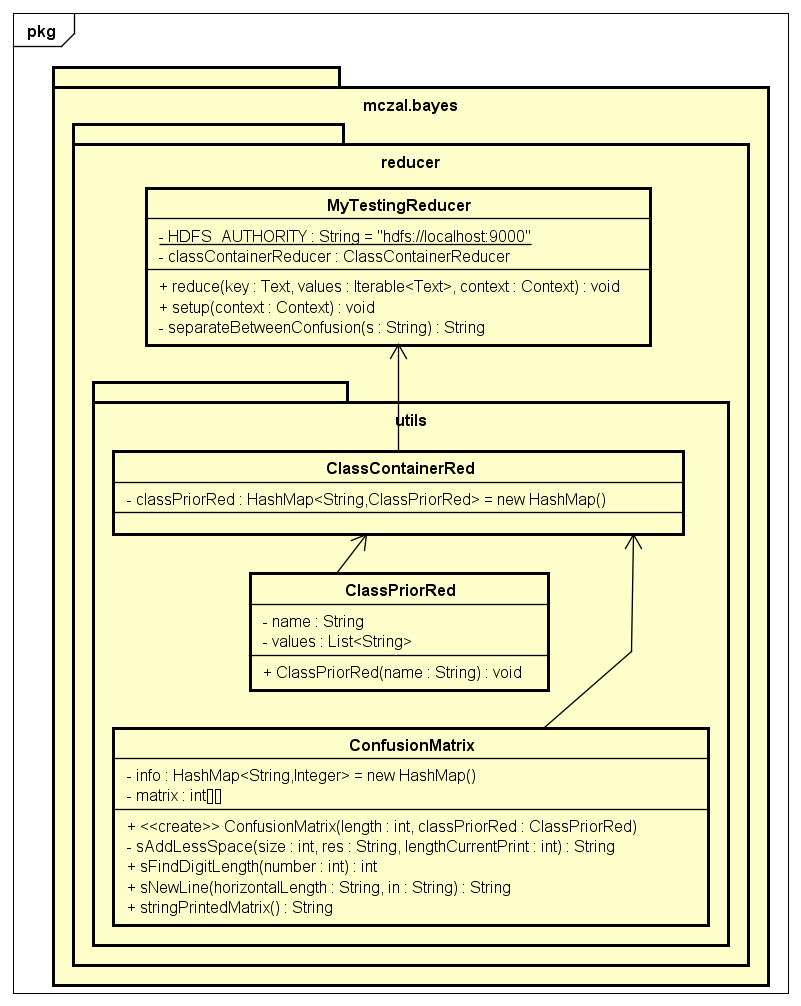
\includegraphics[scale=0.7]{ClassDiagramLengkap/CD_Test_Reducer}
	\caption[Diagram Kelas Modul \textit{Testing: Package Reducer}]{Diagram Kelas Modul \textit{Testing: Package Reducer}}
	\label{fig:Diagram Kelas Modul Testing: Package Reducer}
\end{figure}
Pada package ini terdapat 4 kelas utama yang akan digunakan untuk menjalankan proses \textit{reduce} pada modul \textit{testing}. Sebagian diantaranya berada di dalam \textit{sub-package} yang berbeda. Berikut merupakan penjelasan tiap package dan kelas:

\begin{enumerate}
	\item Kelas \texttt{MyTestingReducer}
	Kelas ini merupakan kelas utama yang akan dijalankan pada proses reduce. Kelas ini memiliki 2 atribut dan 3 operasi yang akan digunakan untuk dapat melakukan operasi pada fase reduce secara keseluruhan. Berikut merupakan penjelasan mengenai atribut dan operasi pada kelas ini:
	\begin{itemize}
		\item{Atribut}
		\begin{enumerate}
			\item{\verb|HDFS_AUTHORITY|}\\
			Atribut ini bertipe \textit{String} dan memiliki \textit{modifier} \textit{static} dan \textit{final} agar nilainya tidak dapat diubah - ubah. Inisialisasi pertama dari atribut ini adalah: \verb|"hdfs://master:9000"|. \verb|"hdfs://master:9000"| merupakan url dari node master yang digunakan untuk dapat berkomunikasi dengan node master pada lingkungan \textit{hadoop}. Atribut ini digunakan untuk \textit{request} operasi baca file \textit{meta.info} dan model NBC pada HDFS.
		
			\item{\texttt{classContainerReducer}}\\
			Atribut ini bertipe \texttt{ClassContainerReducer} yang akan digunakan untuk menyimpan seluruh atribut kelas pada NBC. 
			
		\end{enumerate}
		
		\item{Operasi}
		\begin{enumerate}
			\item{\texttt{reduce()}}\\
			Operasi ini akan melakukan proses pada fase \textit{reduce} untuk proses testing pada modul ini. Proses yang dilakukan akan meliputi perhitungan nilai - nilai pada \texttt{confusion matrix} untuk setiap atribut kelas berdasarkan hasil klasifikasi pada fase \textit{map} sebelumnya. Setelah itu, proses ini juga akan melakukan kalkulasi untuk \textit{error rate}. Variabel yang akan digunakan pada perhitungan \textit{error rate} adalah: (1) \texttt{Accuracy} (2) \texttt{Precision} (3) \texttt{Recall} (4) \texttt{F-Measure}. Berikut merupakan \textit{pseudo-code} untuk proses \textit{reduce} pada modul \textit{testing}:
			\begin{algorithm}[H]
			\caption{NBC Testing algorithm}\label{alg:NBCTestMap}
			\begin{algorithmic}[1]
			\Procedure{Reduce}{$key,values[],context$}\Comment{Reduce function}
			
			\State \verb|HDFS_AUTHORITY| $\gets$ \texttt{"hdfs://master:9000"}
			\State \texttt{classContainerRed} $\gets$ \texttt{ClassContainerRed}

			\State \texttt{classPriorRed = classContainerRed.get[key]}
			\State \texttt{confusionMatrix} $\gets$ \texttt{ConfusionMatrix(classPriorRed.valueSize,classPriorRed)}
			\State \texttt{outKey} $\gets$ \texttt{"@" + key}\Comment{class name}
			
			\ForAll{$s \in values$}
				\State \texttt{splitter} $\gets$ \texttt{s.split("\\|")}
				\State \texttt{actual} $\gets$ \texttt{splitter[2].split("=")[1]}
				\State \texttt{predicted} $\gets$ \texttt{splitter[0].split("=")[1]}
				
				\State \texttt{predIndex} $\gets$ \texttt{confusionMatrix.get(predicted)}
				\State \texttt{actIndex} $\gets$ \texttt{confusionMatrix.get(actual)}
				\State \texttt{confusionMatrix.getMatrix()[actIndex][predIndex]++}
			\EndFor 
        	
        	\State \texttt{outKey} $\gets$ \texttt{confusionMatrix.stringPrintedMatrix()}
			   	
        	\State \texttt{dividend} $\gets 0$ \Comment{Accuracy}
			\State \texttt{divisor}	$\gets 0$
			
			\For{$i \gets 0$ \textbf{to} \texttt{confusionMatrix.matrixLength}}
				\For{$j \gets 0$ \textbf{to} \texttt{confusionMatrix.matrixLength}}
					\If{$i=j$}
						\State \texttt{dividend} $+=$ \texttt{confusionMatrix.getMatrix()[i][j]}
					\EndIf
					\State \texttt{divisor} $+=$ \texttt{confusionMatrix.getMatrix()[i][j]}
				\EndFor
			\EndFor
			
			\State \texttt{accuracyOperator} $\gets$ \texttt{dividend + "/" + divisor}
			\State \texttt{accuracyResult} $\gets$ \texttt{dividend/divisor}
			\State \texttt{outVal} $+=$ \texttt{accuracyOperator+"="+accuracyResult}
			
			\ForAll{\texttt{(className,index)} $\in$ \texttt{confusionMatrix}}

				\State \texttt{currTP} $\gets$ \texttt{confusionMatrix.getMatrix()[index][index]}
				\State \texttt{currFP} $\gets 0$
				\State \texttt{currFN} $\gets 0$
				
				\For{$i \gets 0 $ \textbf{to} \texttt{confusionMatrix.matrixLength}}
					\If{$i != index$}
						\State \texttt{currFP} $+=$ \texttt{confusionMatrix.getMatrix()[i][index]}
						\State \texttt{currFN} $+=$ \texttt{confusionMatrix.getMatrix()[index][i]}
					\EndIf
				\EndFor
				//*\Comment{Precision}
				\State \texttt{precisionOperation} $\gets$ \texttt{currTP + "/" + currTP + "+" + currFP}
				\State \texttt{precisionResult} $\gets$ \texttt{currTP/(currTP + currFP)}
				\State \texttt{outVal} $+=$ \texttt{precisionOperation + "=" + precisionResult}
				
				//*\Comment{Recall}
				\State \texttt{recallOperation} $\gets$ \texttt{currTP + "/" + currTP + " + " + currFN}
				\State \texttt{recallResult} $\gets$ \texttt{currTP/ (currTP + currFN)}
				\State \texttt{outVal} $+=$ \texttt{recallOperation + "=" + recallResult}
				
				//*\Comment{F-Measure}
				\State $\alpha \gets$ \texttt{(2*precisionResult*recallResult) / (precisionResult+recallResult)}
				\State \texttt{fMeasureOperation} $\gets 1 / {alpha{1 / P}+(1-alpha) 1/R}$
				\State \texttt{fMeasureResult} $\gets 1/((alpha * (1/P)) + ((1 - alpha) * (1/R)))$
				\State \texttt{outVal} $+=$ \texttt{fMeasureOperation + "=" + fMeasureResult}
				
				
			\EndFor
			
			\State \texttt{write(outKey,outVal)}
				
			\EndProcedure
			\end{algorithmic}
			\end{algorithm}
			
			\item{\texttt{setup()}}\\
			Operasi ini akan melakukan pembacaan pada model NBC yang sudah dibuat sebelumnya dalam HDFS. Model NBC yang dibaca hanya yang untuk atribut yang bertipe kelas dan lalu memasukkannya ke dalam kelas kontainer pada proses ini.
			
			
			\item{\texttt{separateBetweenConfusionMatrix(s)}}\\
			Operasi ini akan melakukan penambahan pada \textit{string parameter} dengan separator yang ditentukan di dalam operasi ini.
			
		\end{enumerate}
	
		
		
		
	\end{itemize}
	
	\item \texttt{package utils}
	Pada kelas \textit{package} ini	terdapat 3 kelas utama yang digunakan untuk menyimpan atribut kelas dari model NBC dan penyimpanan untuk \texttt{confusion matrix} yang akan digunakan untuk melakukan perhitungan \textit{error rate}. Berikut merupakan penjeleasan kelas - kelas yang terdapat pada \textit{package} ini:
	\begin{enumerate}
		\item \texttt{ClassContainerRed}\\
		Kelas ini akan digunakan sebagai penyimpanan seluruh atribut kelas pada model NBC. Kelas ini memiliki 1 atribut yaitu \texttt{classPriorRed} yang bertipe \texttt{HashMap}. Atribut ini memiliki \texttt{key=String} sebagai nama dari kelas tersebut dan \texttt{value=ClassPriorRed} sebagai kelas yang akan menyimpan detail dari kelas tersebut. Atribut ini akan berisi kumpulan dari atribut kelas pada NBC.
		
		\item \texttt{ClassPriorRed}\\
		Kelas ini akan merepresentasikan atribut kelas pada model NBC yang ada. Kelas ini memiliki 2 atribut, diantaranya adalah:
		\begin{enumerate}
			\item \texttt{name}\\
			Atribut ini akan berisi nama dari atribut kelas model NBC ini.
			
			\item \texttt{values}\\
			Atribut ini akan berisi nilai - nilai diskrit dari atribut kelas model NBC ini.
		\end{enumerate}
		
		\item \texttt{ConfusionMatrix}\\		
		Kelas ini akan merepresentasikan nilai dari \texttt{matrix confusion} yang akan diisi dengan kesesuaian antara hasil prediksi dari algoritma NBC dengan nilai aktual milik record input tersebut. Nilai - nilai dari \texttt{matrix confusion} yang ada pada kelas ini juga akan digunakan untuk melakukan perhitungan \textit{error rate}: (1) \textit{Accuracy}; (2) \textit{Precision}; (3) \textit{Recall}; (4) \textit{F-Measure}. Kelas ini memiliki 2 atribut dan 5 operasi, berikut merupakan penjelasan lebih lanjut:
		\begin{itemize}
			\item Atribut
			\begin{enumerate}
				\item \texttt{info}\\
				Atribut ini bertipe \texttt{HashMap} dengan \texttt{key=string} untuk menyimpan nama dari nilai diskrit pada atribut kelas tertentu dan \texttt{value=integer} untuk menyimpan nomor dari indeks pada matrix yang merepresentasikan kelas tersebut.
			
				\item \texttt{matrix[][]}\\
				Atribut ini bertipe matrix 2 dimensi yang akan merepresentasikan matrix \textit{confusion} dari atribut kelas tertentu.
			
			\end{enumerate}
			
			\item Operasi
			\begin{enumerate}
				\item \texttt{ConfusionMatrix()}\\
				Operasi ini merupakan konstruktor untuk mengisi nilai awal dari dari atribut - atribut pada kelas ini. Operasi ini akan menerima 2 buah parameter yang berisi (1) classPriorRed untuk mencatat tiap nilai diskrit dari atribut kelas tersebut dan (2) panjang dari matrix yang nantinya akan menjadi panjang dari matrix 2 dimensi yang dimiliki oleh kelas ini.
				
				\item \texttt{sAddLessSpace()}\\
				Operasi ini melakukan penambahan spasi pada \textit{string parameter input}. Operasi ini akan digunakan untuk men-\textit{generate} keseluruhan matrix dalam bentuk string	.
				
				\item \texttt{sFindDigitLengthNumber()}\\
				Operasi ini melakukan pencarian panjang digit dari \textit{integer} pada \textit{parameter}. Operasi ini akan digunakan untuk men-\textit{generate} keseluruhan matrix dalam bentuk string.
				
				\item \texttt{sNewLine()}\\
				Operasi ini penambahan baris baru pada \textit{string parameter}. Operasi ini akan digunakan untuk men-\textit{generate} keseluruhan matrix dalam bentuk string.
				
				\item \texttt{stringPrintedMatrix()}\\
				Operasi ini akan melakukan konversi dari matrix 2 dimensi milik atribut \texttt{matrix[][]} ke dalam bentuk \texttt{string} yang nantinya akan di-\textit{print} menjadi keluaran proses ini.
				
			\end{enumerate}					

		\end{itemize}
		
	\end{enumerate}
	
	
\end{enumerate}

\subsection{Diagram Kelas Modul Kelola Input}

Struktur kelas diagram pada modul input dirancang dengan mengikuti \textit{design pattern} milik \textit{Spring Web MVC} yang telah dijelaskan pada landasan teori mengenai \textit{Spring framework} pada \ref{subsec:Spring Framework} dengan tambahan beberapa modifikasi pada layer tengahnya. Berikut merupakan ilustrasi dari package kelas yang akan dirancang pada modul ini:
\begin{figure}[H]
	\centering
	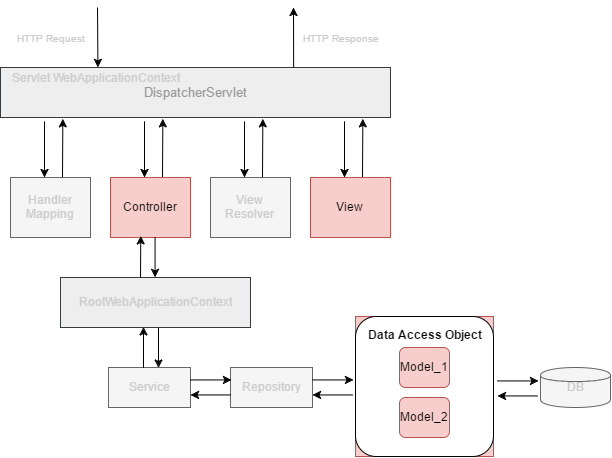
\includegraphics[scale=0.7]{ClassDiagramLengkap/springmvc_rev1}
	\caption[Struktur MVC Pada Modul Kelola Input]{Struktur MVC Pada Modul Kelola Input}
	\label{fig:Struktur MVC Pada Modul Kelola Input}
\end{figure}

Berikut merupakan gambar dari kelas diagram milik modul kelola \textit{input}:
\begin{figure}[H]
	\centering
	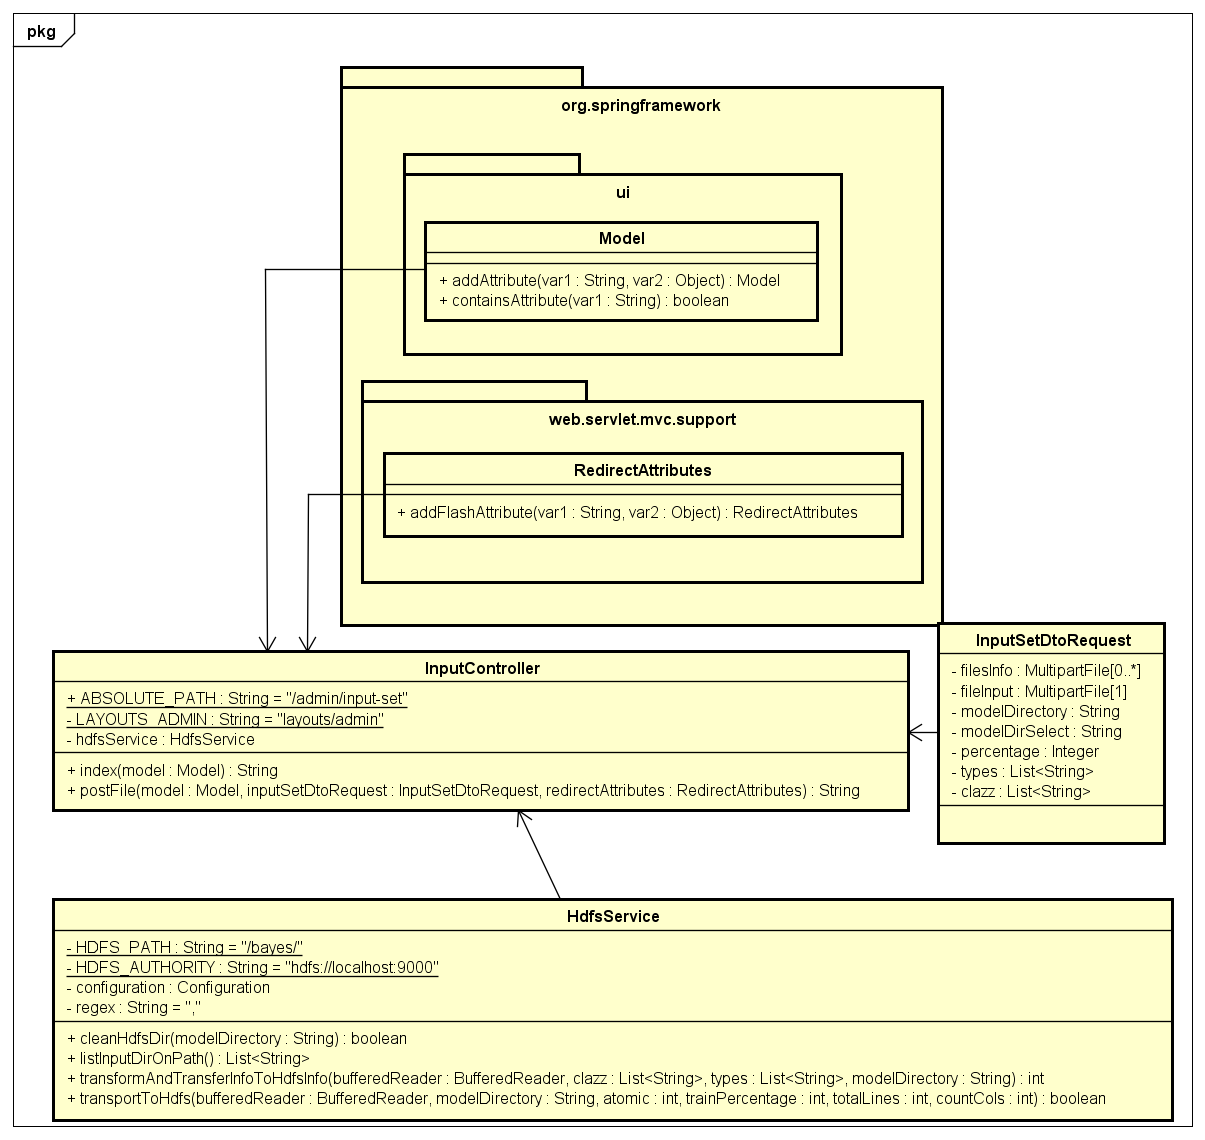
\includegraphics[scale=0.54]{ClassDiagramLengkap/CD_Input}
	\caption[Diagram Kelas Modul Kelola Input]{Diagram Kelas Modul Kelola Input}
	\label{fig:Diagram Kelas Modul Kelola Input}
\end{figure}

Pada modul ini terdapat 3 kelas utama yang akan digunakan untuk melakukan operasi tulis ke dalam HDFS. Selain itu, ada pula 2 kelas milik \textit{springframework} yang digunakan untuk kebutuhan http \textit{request} dan \textit{response} pada \textit{java web servlet}. Berikut merupakan penjelasan kelas - kelas tersebut.
%\begin{enumerate}
\subsubsection{\texttt{InputController}}
	%\item \texttt{InputController}\\
	Kelas ini akan melakukan \textit{handle} request http dari user dan megembalikan \textit{response} yang sesuai dengan apa yang diminta oleh user berkaitan dengan pengelolaan input. Kelas ini akan meneruskan request http dari user ke pada service yang sesuai. Kelas ini memiliki 3 atribut dan 2 operasi, diantaranya adalah:
	%\begin{itemize}
	
	\paragraph{Atribut}
		\begin{enumerate}
			\item \verb|ABSOLUTE_PATH|\\
			Atribut ini bertipe \texttt{string} serta memiliki \textit{modifier static} dan \texttt{final} agar tidak bisa diubah nilai-nya yang akan merepresentasikan path namespace\footnote{\textit{Namespace} merupakan nama pengenal yang unik untuk suatu entitas tertentu.} untuk kelas ini. Atribut ini memiliki nilai inisialisasi awal yang berisi \texttt{"/admin/input-set"}. Jadi, setiap method yang merepresentasikan suatu \textit{request url} dalam kelas ini akan diawali dengan \texttt{"/admin/input-set"}.

			\item \verb|LAYOUTS_ADMIN|\\
			Atribut ini bertipe \texttt{string} serta memiliki \texttt{modifier static} dan \texttt{final} yang akan menyimpan nama view layout dari tampilan html yang akan dirender oleh view. NIlai awal dari atribut ini adalah \texttt{"layouts/admin"}.

			\item \texttt{hdfsService}\\
			Atribut ini bertipe \texttt{HdfsService} yang akan digunakan untuk memanggil operasi operasi yang dienkapsulasi ke dalam layer service. \texttt{HdfsService} akan melakukan request secara lansung kepada node master HDFS untuk melakukan operasi baca dan tulis (\textit{hadoop client}).

		\end{enumerate}
					
	\paragraph{Operasi}
		\begin{enumerate}
			\item \texttt{index(model : Model)}\\
			Operasi ini akan meng-\textit{handle} http request bertipe GET dengan url yang ditentukan pada atribute \verb|ASBOLUTE_PATH| dan akan mengembalikan halaman utama dari modul kelola input ini.
			
			\item \texttt{postFile(inputSetDtoRequest : InputSetDtoRequest,
      redirectAttributes : RedirectAttributes)}\\
			Operasi ini akan meng-\textit{handle} http request bertipe POST dengan url yang ditentukan pada atribute \verb|ASBOLUTE_PATH| dan akan melakukan operasi tulis file ke dalam HDFS. Jika berhasil akan mengembalikan data sukses ke pada html yang akan di-\textit{render} oleh view.

		\end{enumerate}
		
		
	%\end{itemize}	 	

\subsubsection{\texttt{HdfsService}}
		
	Kelas ini merupakan kelas yang akan berhubungan langsung dengan master node pada lingkungan hadoop untuk mengakses HDFS. Kelas ini memiliki 4 atribut dan 4 operasi yang digunakan untuk melakukan operasi baca/tulis ke dalam HDFS. Atribut dan operasi tersebut adalah:
	%\begin{itemize}
	\paragraph{Atribut}
		\begin{enumerate}
			\item \verb|HDFS_PATH|\\
			Atribut ini bertipe \texttt{string} serta memiliki \textit{modifier} \texttt{static} dan \texttt{final} yang akan merepresentasikan \textit{path namespace} pada HDFS yang digunakan oleh keseluruhan perangkat lunak. Atribut ini memiliki nilai inisialisasi awal yang berisi \texttt{"/bayes/"}.

			\item \verb|HDFS_AUTHORITY|\\
			Atribut ini bertipe \texttt{string} serta memiliki \textit{modifier} \texttt{static} dan \texttt{final} yang akan merepresentasikan server authority dari node master HDFS yang digunakan untuk mengakses file - file dalam HDFS. Atribut ini memiliki nilai inisialisasi awal yang berisi \texttt{"hdfs://localhost:9000"}.

			\item \verb|configuration|\\
			Atribut ini bertipe Configuration yang berasal dari \textit{library hadoop}. Atribut ini akan mengatur seluruh konfigurasi yang dibutuhkan untuk dapat melakukan komunikasi dengan lingkungan hadoop untuk dapat mengakses HDFS.

			\item \verb|regex|\\
			Atribut ini akan digunakan untuk pemisah setiap field yang ada dalam tiap baris pada input.
			
		\end{enumerate}				

	\paragraph{Operasi}
		\begin{enumerate}
			\item \texttt{cleanHdfsDir()}\\
			Operasi ini akan melakukan pembersihan seluruh file yang ada pada HDFS dengan url pada parameter yang diberikan. Operasi ini akan mengembalikan true apabila berhasil dan false apabila gagal melakukan komunikasi dengan HDFS.
			
			\item \texttt{listInputDirOnPath()}\\
			Operasi ini akan melakukan pencarian setiap model direktori yang sudah ada pada HDFS. Operasi ini akan mengembalikan tiap model direktori pada HDFS.
			
			\item \texttt{transformAndTransferInfoToHdfsInfo()}\\
			Operasi ini akan melakukan penulisan untuk file info yang telah diinput oleh user sebelumnya untuk dijadikan file \texttt{meta.info} yang disimpan untuk model direktori tertentu pada HDFS. Jika sukses, operasi ini akan mengembalikan jumlah field yang digunakan pada file input yang user masukan.
			
			\item \texttt{transportToHdfs}\\
			Operasi ini akan melakukan penulisan file input yang telah dimasukan oleh user, ke dalam HDFS. Selain itu, operasi ini juga akan menerima presentase yang digunakan pada file yang di-input oleh user untuk dijadikan data training dan data testing. Jika sukses, akan mengembalikan \texttt{boolean} bernilai \textit{true}.
			
		\end{enumerate}
		
	%\end{itemize}
	
	
	\subsubsection{\texttt{InputSetDtoRequest}}
	Kelas ini merupakan kelas DTO\footnote{DTO atau \textit{Command} merupakan salah satu \textit{behavioral pattern} yang melakukan enkapsulasi untuk object yang secara khusus diperuntukkan untuk \textit{object request} dan \textit{object response} dari dan kepada user.} (\textit{Data Transfer Object}) yang diperuntukkan untuk menangani \textit{object request/response} dari dan kepada user dalam proses memasukkan data ke dalam HDFS.


%\end{enumerate}

\subsection{Diagram Kelas Modul Klasifikasi \textit{Naive Bayes}}

Sama seperti pada modul kelola input, struktur kelas diagram pada modul ini juga dirancang dengan mengikuti \textit{design pattern} milik \textit{Spring Web MVC} yang telah dijelaskan pada landasan teori mengenai \textit{Spring framework} pada \ref{subsec:Spring Framework} dengan tambahan beberapa modifikasi pada layer tengahnya. Berikut merupakan ilustrasi dari package kelas yang akan dirancang pada modul ini:
\begin{figure}[H]
	\centering
	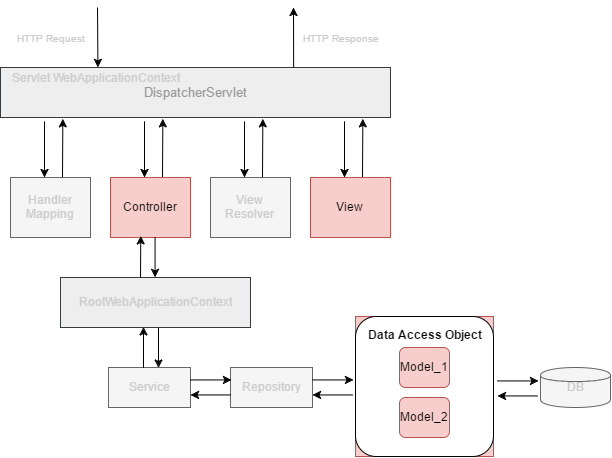
\includegraphics[scale=0.7]{ClassDiagramLengkap/springmvc_rev1}
	\caption[Struktur MVC Pada Modul Klasifikasi]{Struktur MVC Pada Modul Klasifikasi}
	\label{fig:Struktur MVC Pada Modul Klasifikasi}
\end{figure}

Terdapat 3 bagian \textit{layer} yang akan dijelaskan pada kelas diagram modul ini, yaitu (1) \textit{controller}; (2) \textit{service}; (3) \textit{model}. Berikut merupakan penjelasan lebih rinci mengenai tiap \textit{layer} tersebut.

\subsubsection{\textit{Controller}}
\begin{figure}[H]
	\centering
	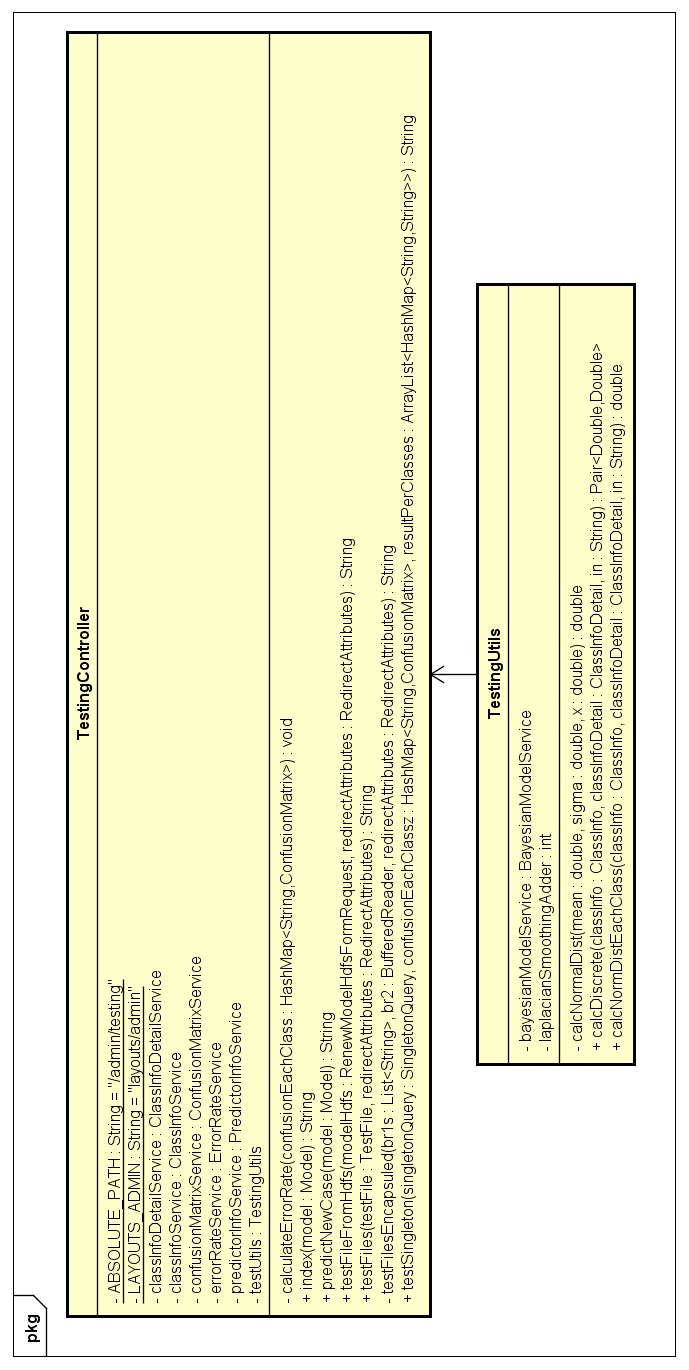
\includegraphics[scale=0.6]{ClassDiagramLengkap/Klasifikasi/Simple_CD_Klasifikasi_Controller_Utils}
	\caption[Diagram Kelas Modul Kelola Input]{Diagram Kelas Modul Kelola Input}
	\label{fig:Diagram Kelas Modul Kelola Input}
\end{figure}

Di dalam \textit{layer controller} terdapat 2 kelas utama sebagai layer yang secara langsung akan menangani request dari user dan memberikan response kepada user. Layer ini menggunakan utility pattern untuk melakukan enkapsulasi perhitungan - perhitungan yang dapat dipisahkan menjadi beberapa bagian operasi tambahan. Kelas tersebut diantara lain adalah:
\begin{enumerate}
	\item \texttt{TestingController}\\
	Kelas ini akan melakukan \textit{handle} request http dari user dan megembalikan \textit{response} yang sesuai dengan apa yang diminta oleh user berkaitan dengan klasifikasi dan \textit{testing} model NBC. Kelas ini akan meneruskan request http dari user ke pada service yang sesuai untuk melakukan klasifikasi maupun \textit{testing}. Kelas ini memiliki 8 atribut dan 7 operasi, diantaranya adalah:
	%\begin{itemize}
	\paragraph{Atribut}
		\begin{enumerate}
			\item \verb|ABSOLUTE_PATH|\\
			Atribut ini bertipe \texttt{string} serta memiliki \textit{modifier static} dan \texttt{final} agar tidak bisa diubah nilai-nya yang akan merepresentasikan path namespace untuk kelas ini. Atribut ini memiliki nilai inisialisasi awal yang berisi \texttt{"/admin/input-set"}. Jadi, setiap method yang merepresentasikan suatu \textit{request url} dalam kelas ini akan diawali dengan \texttt{"/admin/testing"}.

			\item \verb|LAYOUTS_ADMIN|\\
			Atribut ini bertipe \texttt{string} serta memiliki \texttt{modifier static} dan \texttt{final} yang akan menyimpan nama view layout dari tampilan html yang akan dirender oleh view. NIlai awal dari atribut ini adalah \texttt{"layouts/admin"}.


			\item \texttt{classInfoDetailService}\\
			Atribut ini akan merepresentasikan \textit{service} dari nilai - nilai diskrit dari atribut kelas tertentu secara spesifik/detil. \texttt{ClassInfoDetailService} dibuat untuk menyimpan logika program yang berguna untuk menyimpan, memperoleh, dan melakukan pembaharuan terhadap nilai detil dari atribut kelas pada model NBC.

			\item \texttt{classInfoService}\\
			Atribut ini akan merepresentasikan \textit{service} dari atribut kelas pada model NBC secara umum. \texttt{ClassInfoService} dibuat untuk menyimpan logika program yang berguna untuk menyimpan, memperoleh, dan melakukan pembaharuan terhadap atribut kelas yang ada pada model NBC.

			\item \texttt{confusionMatrixService}\\
			Atribut ini akan merepresentasikan \textit{service} matrix \textit{confusion} dari hasil test klasifikasi pada model NBC. \texttt{ConfusionMatrixService} dibuat untuk menyimpan logika program yang berguna untuk menyimpan, memperoleh, dan melakukan pembaharuan yang spesifik terhadap nilai matrix \textit{confusion} serta seluruh kelas yang dicatat di dalamnya.

			\item \texttt{errorRateService}\\
			Atribut ini akan merepresentasikan \textit{service} \textit{error rate} dari hasil test klasifikasi pada model NBC. \texttt{ErrorRateService} dibuat untuk menyimpan logika program yang berguna untuk menyimpan, memperoleh, dan melakukan pembaharuan yang spesifik terhadap nilai - nilai \textit{error rate} pada tiap kelas.

			\item \texttt{predictorInfoService}\\
			Atribut ini akan merepresentasikan \textit{service} dari atribut prediktor pada model NBC secara umum. \texttt{PredictorInfoService} dibuat untuk menyimpan logika program yang berguna untuk menyimpan, memperoleh, dan melakukan pembaharuan terhadap seluruh atribut prediktor yang ada pada model NBC.

			\item \texttt{testingUtils}\\
			Atribut ini bertipe \textit{TestingUtils} yang akan melakukan enkapsulasi untuk beberapa operasi yang dilakukan pada kelas \texttt{TestingController}. Sehingga, program dapat lebih mudah dibaca.

		\end{enumerate}
		
	\paragraph{Operasi}
		\begin{enumerate}
			\item \texttt{- calculateErrorRate(confusionEachClass : HashMap<String,ConfusionMatrix>): void}\\
			Operasi ini akan melakukan perhitungan \textit{error rate} untuk (1) \textit{Accuracy}; (2) \textit{Precision}; (3) \textit{Recall}; (4) \textit{F-Measure}, yang dihasilkan dari pengolahan matrix \textit{confusion} dan akan menerima parameter matrix \textit{confusion} untuk mengkalkulasi nilai TP \textit{(true positive)}, FP \textit{(false positive)} TN \textit{(true negative)} FN \textit{(false negative)}. Setelah hasil didapat,  akan langsung melakukan penyimpanan ke dalam \textit{database}.
			
			\item \texttt{+ index(model : Model): String}\\
			Operasi ini akan meng-\textit{handle} http request bertipe GET dengan url yang ditentukan pada atribute \verb|ASBOLUTE_PATH| dan akan mengembalikan halaman utama dari modul klasifikasi ini.

			\item \texttt{+ predictNewCase(model : Model): String}\\
			Operasi ini akan meng-\textit{handle} http request bertipe GET dengan url \verb|ASBOLUTE_PATH+"/predict-new-case"| dan akan mengembalikan halaman untuk melakukan klasifikasi untuk 1 kasus.

			\item \texttt{+ testFileFromHdfs(modelHdfs : RenewModelHdfsFormRequest, redirectAttributes : RedirectAttributes): String}\\
			Operasi ini akan meng-\textit{handle} http \textit{request} bertipe POST dengan url \verb|ASBOLUTE_PATH+"/files-from-hdfs"| dan akan menerima parameter \texttt{modelHdfs} bertipe \texttt{RenewModelHdfsFormRequest} yang akan diisi dengan keterangan path file yang ada dalam HDFS. Setelah menerima \textit{request}, operasi ini akan meneruskan-nya ke pada \texttt{hdfsService} untuk dilakukan proses klasifikasi dengan data yang sudah ada di dalam HDFS. 

			\item \texttt{+ testFiles(testFile : TestFile, redirectAttributes : RedirectAttributes): String}\\
			Operasi ini akan meng-\textit{handle} http \textit{request} bertipe POST dengan url \verb|ASBOLUTE_PATH+"/files"| dan akan menerima parameter \texttt{testFile} bertipe \texttt{TestFile} yang akan berisi mengenai seluruh file dan keterangan lainnya untuk melakukan testing. Setelah menerima \textit{request} akan langsung melakukan perhitungan untuk setiap file yang diinput oleh user. 


			\item \texttt{- testFilesEncapsuled(br1s : List<String>, br2 : BufferedReader, redirectAttributes : RedirectAttributes): String}\\
			Operasi ini merupakan enkapsulasi dari proses testing pada operasi \texttt{testFiles()} dan akan melakukan test pada model NBC untuk setiap file yang diterima pada parameter.


			\item \texttt{+ testSingleton(singletonQuery : SingletonQuery, confusionEachClassz : HashMap<String,ConfusionMatrix>, resultPerClasses : ArrayList <HashMap <String,String>>) : String}\\
			Setiap operasi testing pada modul ini akan memanggil operasi ini. Operasi ini akan melakukan perhitungan klasifikasi untuk tiap satu baris/\textit{record} dari file input. Hampir seluruh pemanggilan operasi - operasi lain untuk membantu melakukan perhitungan klasifikasi model NBC pada atribut \texttt{testingUtils} yang bertipe \texttt{TestingUtils} berada pada operasi ini.

		\end{enumerate}
		
	%\end{itemize}
	
	\item \texttt{TestingUtils}\\
	Kelas ini merupakan kelas yang meng-enkapsulasi beberapa operasi yang dilakukan pada kelas \texttt{TestingController} agar membuat kode program bisa lebih mudah dibaca dan dapat digunakan kembali oleh operasi - operasi lain yang membutuhkan perhitungan yang disediakan oleh kelas ini. Kelas ini memiliki 2 atribut dan 3 operasi, diantaranya adalah:
	%\begin{itemize}
	\paragraph{Atribut}
		\begin{enumerate}
			\item \texttt{bayesianModelService}\\
			Atribut ini bertipe \texttt{BayesianModelService} yang akan digunakan untuk memanggil operasi operasi yang dienkapsulasi ke dalam layer service untuk langsung melakukan koneksi ke dalam database milik \textit{BayesianModel}. \texttt{BayesianModelService}.
			
		\end{enumerate}				

	\paragraph{Operasi}
		\begin{enumerate}
			\item \texttt{- calcNormalDist}\\
			Operasi ini akan membantu operasi pada \texttt{calcNormDistEachClass} untuk menghitung fungsi normal distribusi dari parameter yang diberikan
			
			\item \texttt{+ calcDiscrete}\\
			Operasi ini akan membantu \texttt{TestingController} dalam melakukan proses klasifikasi untuk menghitung probabilitas posterior atribut yang bertipe disrkit.

			\item \texttt{- calcNormDistEachClass}\\
			Operasi ini akan membantu \texttt{TestingController} dalam melakukan proses klasifikasi untuk menghitung probabilitas posterior atribut yang bertipe numerik dengan menghitung normal distribusi dari atribut tersebut.

		\end{enumerate}
		
		
	%\end{itemize}


\end{enumerate}
	

\subsubsection{\textit{Service}}
\begin{figure}[H]
	\centering
	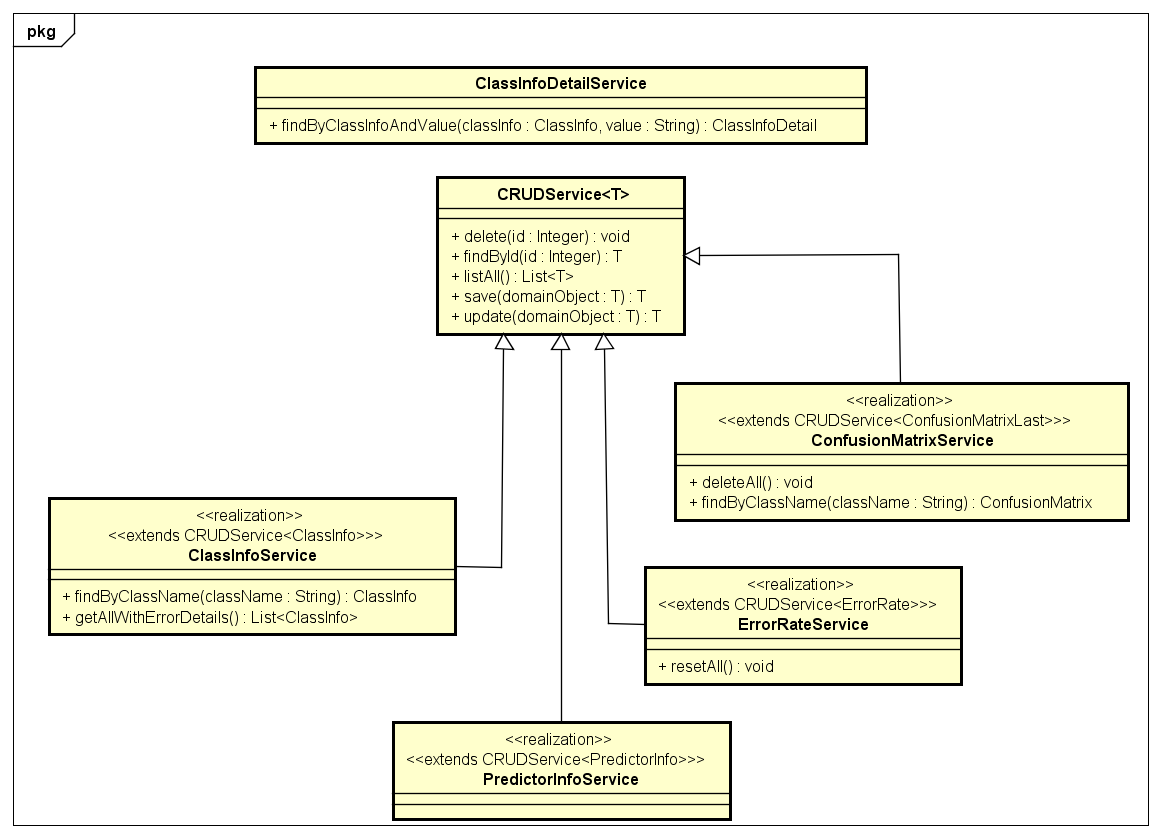
\includegraphics[scale=0.55]{ClassDiagramLengkap/Klasifikasi/Simple_CD_Klasifikasi_Services}
	\caption[Diagram Kelas Modul Kelola Input]{Diagram Kelas Modul Kelola Input}
	\label{fig:Diagram Kelas Modul Kelola Input}
\end{figure}
\textit{Layer service} pada modul ini menggunakan konsep \textit{polymorphism}\footnote{
\textit{Polymorphism} merupakan 1 dari 3 mekanisme dalam OOP (\textit{Object Oriented Programming}) untuk men-\textit{general}-kan beberapa \textit{method} yang secara umum memiliki tujuan yang sama tetapi berbeda implementasi-nya \cite{AbsoluteJava:2012}.} pada java untuk menghindari terjadinya redundansi kode yang memiliki tujuan sama. Berikut merupakan penjelasan lebih rinci mengenai kelas - kelas pada \textit{layer} ini:

\begin{enumerate}
	\item \texttt{CRUDService}\\
	Kelas ini merupakan \textit{base class} sebagian besar kelas service lainnya dan memiliki \textit{generic type} \texttt{T} yang perlu diberikan untuk tiap kelas yang menjadi \textit{descendant}-nya. Terdapat 5 \textit{method} abstrak yang dimiliki oleh kelas ini, \textit{method - method} tersebut diantara lain adalah:
	\begin{enumerate}
		\item \texttt{delete(id: Integer): void}\\
		\textit{Method} ini merupakan \textit{method} abstrak yang perlu diimplementasikan oleh seluruh kelas yang menjadi turunan dari kelas ini dan akan melakukan penghapusan \textit{object} bertipe \texttt{T} yang memiliki \texttt{id} pada parameter masukan \textit{method} ini.
		
		\item \texttt{findById(id: Integer): T}\\
		\textit{Method} ini merupakan \textit{method} abstrak yang perlu diimplementasikan oleh seluruh kelas yang menjadi turunan dari kelas ini dan akan melakukan pencarian \textit{object} bertipe \texttt{T} yang memiliki \texttt{id} pada parameter masukan \textit{method} ini.

		\item \texttt{listAll(): List<T>}\\
		\textit{Method} ini merupakan \textit{method} abstrak yang perlu diimplementasikan oleh seluruh kelas yang menjadi turunan dari kelas ini dan akan melakukan pengambilan seluruh \textit{object} bertipe \texttt{T} pada \textit{database}.

		\item \texttt{save(domainObject: T): T}\\
		\textit{Method} ini merupakan \textit{method} abstrak yang perlu diimplementasikan oleh seluruh kelas yang menjadi turunan dari kelas ini dan akan melakukan pembuatan \textit{object} baru bertipe \texttt{T} dan memasukkannya ke dalam \textit{database}.

		\item \texttt{update(domainObject: T): T}\\
		\textit{Method} ini merupakan \textit{method} abstrak yang perlu diimplementasikan oleh seluruh kelas yang menjadi turunan dari kelas ini dan akan melakukan perbaharuan \textit{object} bertipe \texttt{T} dan melakukan \textit{update} ke dalam \textit{database}.
		
	\end{enumerate}
	
	\item \texttt{PredictorInfoService}\\
	Kelas ini merupakan kelas \textit{service} turunan dari kelas \texttt{CRUDService} yang akan menangani proses baca tulis ke dalam database pada \textit{object} yang bertipe \texttt{PredictorInfo}. Sehingga, secara langsung akan memiliki juga operasi - operasi pada \textit{base class} tersebut. 
	
	\item \texttt{ConfusionMatrixService}\\
	Kelas ini merupakan kelas \textit{service} turunan dari kelas \texttt{CRUDService} yang akan menangani proses baca tulis ke dalam database pada \textit{object} yang bertipe \texttt{PredictorInfo}. Sehingga, secara langsung akan memiliki juga \textit{operasi - operasi} pada \textit{base class} tersebut. Kelas ini memiliki beberapa operasi tambahan yang diperlkan khusus untuk kelas \texttt{ConfusionMatrixService}.
	\begin{enumerate}
		\item \texttt{deleteAll()} akan melakukan penghapusan seluruh record/model yang merepresentasikan \textit{object} instansiasi dari kelas ini.
		\item \texttt{findByClassName(name: String)} akan melakukan pencarian \textit{object} instansiasi dari kelas ini dengan memberikan nama atribut kelas sebagai parameter masukan.
	\end{enumerate}
	
	\item \texttt{ErrorRateService}\\
	Kelas ini merupakan kelas \textit{service} turunan dari kelas \texttt{CRUDService} yang akan menangani proses baca tulis ke dalam database pada \textit{object} yang bertipe \texttt{ErrorRate}. Sehingga, secara langsung akan memiliki juga \textit{operasi - operasi} pada \textit{base class} tersebut. Kelas ini memiliki 1 operasi tambahan yang diperlukan khusus untuk kelas \texttt{ErrorRateService}, yaitu \texttt{resetAll()} yang akan melakukan penghapusan seluruh instansiasi dari \textit{object} \textit{ErrorRate} di dalam \textit{database} yang sudah ada sebelumnya.
	
	\item \texttt{ClassInfoService}\\
	Kelas ini merupakan kelas \textit{service} turunan dari kelas \texttt{CRUDService} yang akan menangani proses baca tulis ke dalam database pada \textit{object} yang bertipe \texttt{ErrorRate}. Sehingga, secara langsung akan memiliki juga \textit{operasi - operasi} pada \textit{base class} tersebut. Kelas ini memiliki beberapa operasi tambahan yang diperlukan khusus untuk kelas \texttt{ClassInfoService}.
	\begin{enumerate}
		\item \texttt{findByClassName(className: String): ClassInfo} akan melakukan pencarian untuk instansiasi \textit{object} pada kelas ini dalam \textit{database} dengan parameter masukan nama kelas.
		\item \texttt{getAllWithErrorDetails(): List<ClassInfo>} akan mengembalikan seluruh instansiasi dari \textit{object} \texttt{ClassInfo} dengan mengikutsertakan relasi - relasi yang dimiliki tiap \textit{object} dengan kelas \texttt{ErrorRate}.
	\end{enumerate}
	
	\item \texttt{ClassInfoDetailService}\\
	Kelas ini merupakan satu - satunya kelas \textit{service} yang bukan merupakan turunan dari kelas \texttt{CRUDService}. Kelas ini dibuat khusus untuk pencarian detil dari atribut kelas spesifik dan akan melakukan update terhadap \textit{errorRate} yang merupakan relasi dari instansiasi \textit{object} kelas \texttt{ClassInfoDetail}. Operasi yang dimiliki pada kelas ini adalah \texttt{findByClassInfoAndValue(classInfo: ClassInfo, value: String): CLassInfoDetail}, yang akan mengembalikan instansiasi dari \textit{object} kelas ini dengan parameter masukan object kelas info serta nama dari nilai diskrit \textit{object} kelas tersebut. 

\end{enumerate}

\subsubsection{\textit{Model}}
\begin{figure}[H]
	\centering
	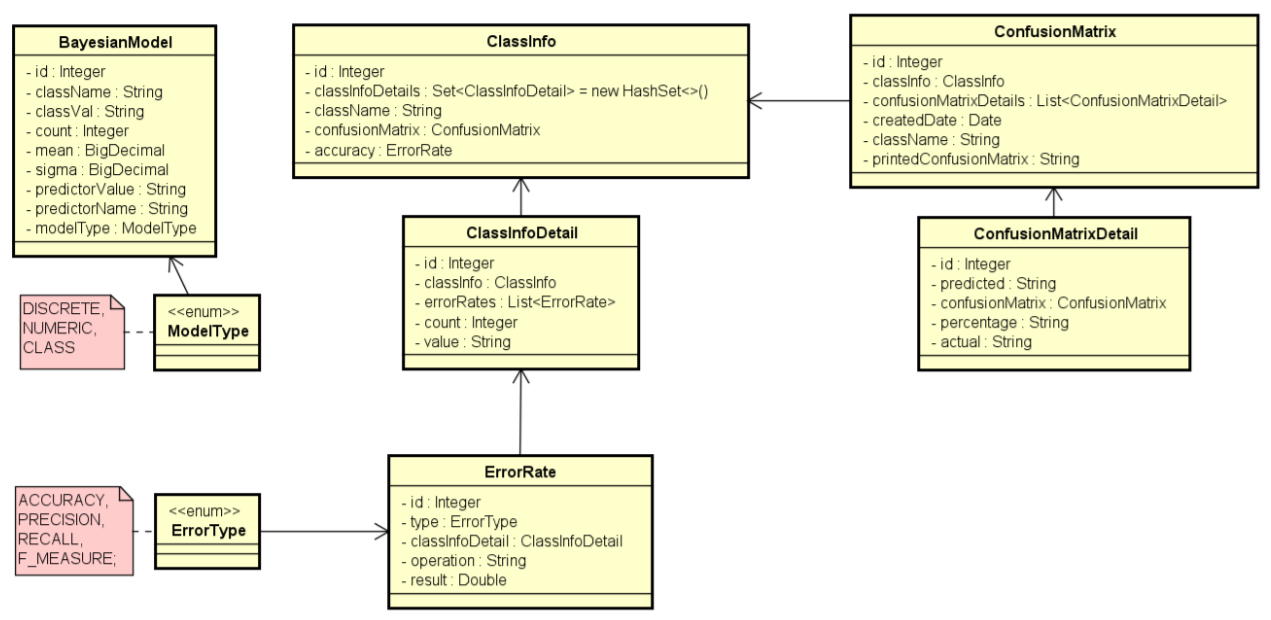
\includegraphics[scale=0.6]{ClassDiagramLengkap/Klasifikasi/Simple_CD_Klasifikasi_Model}
	\caption[Diagram Kelas Modul Kelola Input]{Diagram Kelas Modul Kelola Input}
	\label{fig:Diagram Kelas Modul Kelola Input}
\end{figure}

\textit{Layer model} akan merepresentasikan seluruh \textit{object} model yang dimiliki pada modul ini dan juga akan sekaligus merepresentasikan entitas-entitas/tabel-tabel yang ada pada modul. Layer ini memanfaatkan fitur ORM\footnote{\textit{Spring} menyediakan integrasi dengan \textit{Hibernate, JPA(Java Pesistence API), dan JDO(Java Data Objects)} untuk melakukan pemodelan object milik java dengan model pada DBMS serta relasi - relasi yang dibutuhkan pada DBMS} (\textit{Object Relational Model}) milik \textit{spring framework} yang akan mengatasi seluruh transformasi dari object pada java ke model pada DBMS. Kelas - kelas pada layer ini merupakan kelas POJO pada java. Berikut merupakan penjelasan lebih rinci mengenai kelas - kelas pada \textit{layer} ini:

\begin{enumerate}
	\item \texttt{ConfusionMatrix}\\
	Kelas model ini akan merepresentasikan matrix \textit{confusion} yang digunakan untuk melakukan perhitungan hasil klasifikasi dari suatu data \textit{testing}. Kelas ini memiliki 6 atribut, diantaranya adalah:
	\begin{enumerate}
		\item \texttt{id}, bertipe \textit{integer} digunakan sebagai atribut unik untuk pengenal setiap instansiasi dari \textit{object} kelas ini.

		\item \texttt{classInfo}, bertipe \texttt{ClassInfo} merupakan relasi 1-ke-1 dengan kelas ini. Setiap matrix \textit{confusion} akan memiliki 1 atribut kelas info dan begitu juga sebaliknya.
	
		\item \texttt{confusionMatrixDetails}, bertipe \texttt{List <ConfusionMatrixDetail>} merupakan relasi \textit{1-to-many} dengan kelas ini. \texttt{confusionMatrixDetails} akan menyimpan seluruh keterangan detail mengenai tiap matrix \textit{confusion}.

		\item \texttt{createdDate}, bertipe \texttt{Date} akan mencatat waktu \textit{timestamp} \textit{object} instansiasi dari kelas ini dibuat.		

		\item \texttt{className}, bertipe \texttt{String} sebagai nama atribut kelas dari instansiasi \textit{object} kelas ini.

		\item \texttt{printedConfusionMatrix}, bertipe \texttt{String} akan merepresentasikan suatu matrix dari kelas ini dalam bentuk \texttt{string}.

	\end{enumerate}		
	
	\item \texttt{ConfusionMatrixDetail}\\
	Kelas model ini akan merepresentasikan detil dari atribut matrix \textit{confusion}. Kelas ini memiliki 5 atribut, diantaranya adalah:
	\begin{enumerate}
		\item \texttt{id}, bertipe \textit{integer} digunakan sebagai atribut unik untuk pengenal setiap instansiasi dari \textit{object} kelas ini.
				

		\item \texttt{predicted}, bertipe \textit{string} digunakan untuk mencatat hasil nilai prediksi kelas pada klasifikasi yang telah ditentukan.
		

		\item \texttt{confusionMatrix}, bertipe \texttt{ConfusionMatrix} merupakan relasi \textit{many-to-1} dengan kelas ini.

		\item \texttt{percentage}, bertipe \texttt{string} merupakan presentase dominasi hasil nilai atribut kelas yang diprediksi dari proses klasifikasi.
		

		\item \texttt{actual}, bertipe \textit{string} digunakan untuk mencatat hasil nilai kelas asli pada data yang dimasukkan ke dalam algoritma klasifikasi \textit{naive bayes}.

	\end{enumerate}


	\item \texttt{ClassInfo}\\
	Kelas model ini akan merepresentasikan atribut kelas pada model NBC yang ada. Kelas ini memiliki 5 atribut, diantaranya adalah:
	\begin{enumerate}
		\item \texttt{id}, bertipe \textit{integer} digunakan sebagai atribut unik untuk pengenal setiap instansiasi dari \textit{object} kelas ini.
		
		\item \texttt{classInfoDetails}, bertipe \texttt{Set<ClassInfoDetails>} merepresentasikan kumpulan tiap nilai-diskrit detil dari atribut kelas NBC ini.
		
		\item \texttt{className}, bertipe \texttt{string} merupakan nama dari atribut kelas ini pada NBC.
		
		\item \texttt{confusionMatrix}, bertipe \texttt{ConfusionMatrix} merupakan relasi 1-ke-1 dengan kelas ini. Setiap instansiasi dari \textit{object} \textit{ClassInfo} akan memiliki 1 atribut \texttt{confusionMatrix} dan begitu juga sebaliknya.
		
		\item \texttt{accuracy}, bertipe \texttt{ErrorRate} merupakan hasil \textit{error rate} bertipe \textit{accuracy} setelah klasifikasi dilakukan.
		
		
	\end{enumerate}

	\item \texttt{ClassInfoDetail}\\
	Kelas model ini akan merepresentasikan detil dari atribut kelas pada kelas \texttt{ClassInfo}. Kelas ini memiliki 5 atribut, diantaranya adalah:
	\begin{enumerate}
		\item \texttt{id}, bertipe \textit{integer} digunakan sebagai atribut unik untuk pengenal setiap instansiasi dari \textit{object} kelas ini.
		
		\item \texttt{classInfo}, bertipe \texttt{ClassInfo} merupakan relasi many-to-1 dari kelas ini ke kelas \texttt{ClassInfo}.
		
		\item \texttt{errorRates}, bertipe \texttt{List<ErrorRate>} merupakan kumpulan \textit{error rate} yang dimiliki oleh atribut ini. Kumpulan \textit{error rate} tersebut bisa bertipe: (1)\textit{precision}; (2)\textit{recall}; (3)\textit{f-measure}.
				
		\item \texttt{count}, bertipe \textit{integer} merupakan jumlah frekuensi kemunculan atribut kelas yang bernilai tertentu pada NBC.

		\item \texttt{value}, bertipe \textit{string} merupakan nama dari nilai-diskrit atribut kelas tertentu pada NBC.
		
	\end{enumerate}

	\item \texttt{ErrorRate}\\
	Kelas model ini akan merepresentasikan nilai - nilai perhitungan \textit{error rate} yang dihasilkan setelah proses klasifikasi pada data \textit{testing} dilakukan. Kelas ini memiliki 5 atribut, diantaranya adalah:
	\begin{enumerate}
		\item \texttt{id}, bertipe \textit{integer} digunakan sebagai atribut unik untuk pengenal setiap instansiasi dari \textit{object} kelas ini.
		
		\item \texttt{type}, bertipe \textit{ErrorType} merupakan tipe \textit{error rate} pada \textit{object} instansiasi dari kelas ini. 
		
		\item \texttt{classInfoDetail}, bertipe \textit{ClassInfoDetail} merupakan relasi \textit{many-to-1} ke kelas \texttt{ClassInfoDetail}. Sehingga, setiap instansiasi dari kelas ini akan memiliki relasi dengan 1 instansiasi dari kelas \texttt{ClassInfoDetail}.
		
		\item \texttt{operation}, bertipe \textit{string} akan digunakan sebagai pencatat operasi yang dilakukan untuk memperoleh hasil pada atribut \textit{result}. Atribut ini dibuat untuk memudahkan user dalam melihat kalkulasi perhitungan sebenarnya pada program dalam menguji kebenaran program.
		
		\item \texttt{result}, bertipe \textit{Double} merupakan nilai dari hasil perhitungan \textit{error rate} pada tipe yang spesifik.
		
		
	\end{enumerate}

	\item \texttt{ErrorType}\\
	\texttt{ErrorType} merupakan \textit{enum} yang merepresentasikan tipe - tipe error pada kelas \texttt{ErrorRate}. \textit{Enum} pada kelas ini berisi:
	\begin{itemize}
		\item \texttt{ACCURACY}
		\item \texttt{PRECISION}
		\item \texttt{RECALL}
		\item \texttt{F-MEASURE}
	\end{itemize}	 

	\item \texttt{PredictorInfo}\\
	Kelas model ini akan merepresentasikan atribut prediktor pada model NBC yang ada. Atribut prediktor tersebut bisa memiliki tipe numerik atau diskrit. Kelas ini memiliki 4 atribut, diantaranya adalah:
	\begin{enumerate}
		\item \texttt{id}, bertipe \textit{integer} digunakan sebagai atribut unik untuk pengenal setiap instansiasi dari \textit{object} kelas ini.
		
		\item \texttt{predictorInfoDetail}, bertipe \textit{Set<PredictorInfoDetail>} akan berguna untuk mencatat seluruh kumpulan detil dari instansiasi kelas ini.

		\item \texttt{predictorName}, bertipe \textit{String} merupakan nama dari atribut prediktor NBC pada kelas ini.
		
		\item \texttt{modelType}, bertipe \textit{ModelType} berguna untuk memberitahu tipe model atribut-NBC dari kelas ini.
		
				
	\end{enumerate}

	\item \texttt{PredictorInfoDetail}\\
	Kelas model ini akan merepresentasikan detil dari atribut kelas pada kelas \texttt{PredictorInfo}. Kelas ini memiliki 9 atribut, diantaranya adalah:
	\begin{enumerate}
		\item \texttt{id}, bertipe \textit{integer} digunakan sebagai atribut unik untuk pengenal setiap instansiasi dari \textit{object} kelas ini.
		
		\item \texttt{classPriorName}, bertipe \textit{String} merepresentasikan nama dari kelas prior yang memiliki hubungan pada perhitungan probabilitas posterior dengan instansiasi dari kelas prediktor ini.
		
		\item \texttt{classPriorValue}, bertipe \textit{String} merepresentasikan nilai-diskrit dari atribut kelas prior yang memiliki hubungan pada perhitungan probabilitas posterior dengan instansiasi dari kelas prediktor ini.
		
		\item \texttt{count}, bertipe \textit{Integer} merupakan jumlah frekuensi kemunculan instansiasi dari kelas ini terhadap atribut \texttt{classPriorValue}.
		
		\item \texttt{mean}, bertipe \textit{Double} merepresentasikan rata - rata dari atribut numerik pada NBC.
		
		\item \texttt{sigma}, bertipe \textit{Double} merepresentasikan nilai sigma/standard-deviasi dari atribut numerik pada NBC.
		
		\item \texttt{predictorInfo}, bertipe \textit{String} merepresentasikan nama atribut prediktor pada NBC.
		
		\item \texttt{value}, bertipe \textit{String} merepresentasikan nilai-diskrit dari atribut prediktor pada model NBC.
		
		
	\end{enumerate}

	\item \texttt{BayesianModel}\\
	Kelas model ini merupakan representasi dari model NBC yang telah dibuat sebelumnya. Kelas ini memiliki 5 atribut, diantaranya adalah:
	\begin{enumerate}
		\item \texttt{id}, bertipe \textit{integer} digunakan sebagai atribut unik untuk pengenal setiap instansiasi dari \textit{object} kelas ini.
		
		\item \texttt{className}, bertipe \textit{String} merepresentasikan nama dari kelas prior yang memiliki hubungan pada perhitungan probabilitas posterior dengan instansiasi dari kelas prediktor ini.

		\item \texttt{classVal}, bertipe \textit{String} merepresentasikan nilai-diskrit dari atribut kelas prior yang memiliki hubungan pada perhitungan probabilitas posterior dengan instansiasi dari kelas prediktor ini.
		
		\item \texttt{count}, bertipe \textit{Integer} merupakan jumlah frekuensi kemunculan instansiasi dari kelas ini terhadap atribut \texttt{classVal}.
		
		\item \texttt{mean}, bertipe \textit{Double} merepresentasikan rata - rata dari atribut numerik pada NBC.
		
		\item \texttt{sigma}, bertipe \textit{Double} merepresentasikan nilai sigma/standard-deviasi dari atribut numerik pada NBC.
		
		\item \texttt{predictorValue}, bertipe \textit{String} merepresentasikan nilai-diskrit dari atribut prediktor pada model NBC.
		
		\item \texttt{predictorName}, bertipe \textit{String} merepresentasikan nama atribut prediktor pada NBC.
		
		\item \texttt{modelType}, bertipe \textit{ModelType} berguna untuk memberitahu tipe model atribut-NBC dari kelas ini.
		
		
	\end{enumerate}

	\item \texttt{ModelType}\\
	\texttt{ModelType} merupakan \textit{enum} yang merepresentasikan tipe - tipe dari atribut prediktor pada kelas \texttt{PredictorInfo}. \textit{Enum} pada kelas ini berisi:
	\begin{itemize}
		\item \texttt{DISCRETE}
		\item \texttt{NUMERIC}
		\item \texttt{CLASS}
	\end{itemize}

\end{enumerate}



